% IIT Delhi BTP Project Report: structure aligned with BTP_Report_Format.docx
% Body text: Times New Roman 12pt equivalent; A4; 1 in margins (matching template sectPr)
\documentclass[12pt,a4paper,oneside]{report}

\usepackage[T1]{fontenc}
% UTF-8 is the engine default for modern TeX (tectonic, pdfTeX in TeX Live); loading inputenc only emits a harmless warning.
\usepackage{mathptmx}
\usepackage{mathtools}
\usepackage{amssymb}
\usepackage{booktabs}
\usepackage{multirow}
\usepackage{longtable}
\usepackage{caption}
\captionsetup{justification=raggedright,singlelinecheck=false}
\usepackage{graphicx}
\usepackage{siunitx}
\usepackage{xurl}
\makeatletter
\g@addto@macro\UrlBreaks{\do\/\do\_}
\makeatother
\usepackage[margin=1in]{geometry}
\usepackage{setspace}
\setstretch{1.5}
\emergencystretch=2.5em
\usepackage{microtype}
\usepackage{titlesec}
\usepackage[numbers,sort&compress]{natbib}
\renewcommand{\bibfont}{\raggedright\sloppy}
\usepackage{tocloft}
\usepackage{enumitem}
\usepackage[hidelinks]{hyperref}

% List of Equations (department sample TOC includes this entry).
% Equation titles are written via manual \addcontentsline after each equation in the body/SI.
\newcommand{\listequationname}{List of Equations}
\newlistof{eqloe}{loe}{\listequationname}

% Centered, numbered chapter titles (analogous to Word ``Heading 1'' in BTP_Report_Format.docx)
\titleformat{\chapter}[display]
  {\normalfont\bfseries\centering}
  {\chaptertitlename\ \thechapter}{12pt}{\large}

\graphicspath{{../figures/}}
\sisetup{detect-all}

% Build from ``paper/``: tectonic --reruns 8 COMPASS_BTP_REPORT.tex (extra passes settle ToC/LoF/bibliography)
%        OR  pdflatex + bibtex + pdflatex ×2
\begin{document}
\hypersetup{pdftitle={COMPASS: Conformation-Map Optimized Mutant Prioritized Adaptive Sequential Sampling},pdfauthor={Anmol Goel}}
% Avoid duplicate PDF named destinations on the title page (xdvipdfmx: @page.1 already defined).
\hypersetup{pageanchor=false}

% === Title page (mirrors BTP template layout)
\begin{titlepage}
\centering
% IIT Delhi logo only. The Word template also unpacked image2--image4 (tiny demo plots from
% the template document, not institute branding); those are omitted here.

\includegraphics[height=2.0cm]{btp_template_assets/image1.png}\par
\vspace*{1.0cm}
{\Large\bfseries COMPASS: Conformation-Map Optimized Mutant Prioritized Adaptive Sequential Sampling\par}
\vspace{0.4cm}
{\large Transferring Source MD Landscapes to Guide Adaptive Seeding of Related Mutants\par}
\vspace{1.2cm}
{\large A PROJECT REPORT\par}
\vspace{0.8cm}
{\normalsize Submitted as part of BBD452 BTech Major Project (BB1)\par}
\vfill
{\normalsize\textbf{Submitted by:} Anmol Goel \quad (Entry No.\ 2022BB11000)\par}
\vspace{0.6cm}
{\normalsize\textbf{Guided by:} Prof.\ Ishaan Gupta\par}
\vspace{1.4cm}
{\normalsize\textbf{DEPARTMENT OF BIOCHEMICAL ENGINEERING AND BIOTECHNOLOGY}\par
{\normalsize INDIAN INSTITUTE OF TECHNOLOGY DELHI\par}}
\vspace{1cm}
{\normalsize May 5, 2026\par}
\vspace*{1.2cm}
\end{titlepage}

\hypersetup{pageanchor=true}
\pagenumbering{roman}
\setcounter{page}{2}

% === Declaration
\phantomsection
\chapter*{Declaration}
\addcontentsline{toc}{chapter}{Declaration}

I certify that
\begin{enumerate}[label=\alph*), itemsep=0.45ex]
\item The work contained in this report is original and has been done by me under the guidance of my supervisor.
\item I have followed the guidelines provided by the Department in preparing the report.
\item I have conformed to the norms and guidelines given in the Honor Code of Conduct of the Institute.
\item Whenever I have used materials (data, theoretical analysis, figures, and text) from other sources, I have given due credit to them by citing them in the text of the report and giving their details in the references. Further, I have taken permission from the copyright owners of the sources, whenever necessary.
\end{enumerate}

\vspace{1.5cm}
\noindent\textbf{Signed by:}\\[0.5em]
Anmol Goel

\cleardoublepage

% === Certificate
\phantomsection
\chapter*{Certificate}
\addcontentsline{toc}{chapter}{Certificate}

It is certified that the work contained in this report titled ``COMPASS: Conformation-Map Optimized Mutant Prioritized Adaptive Sequential Sampling'' is the original work done by Anmol Goel and has been carried out under my supervision.

\vspace{1.5cm}
\noindent\textbf{Signed by:}\\[1.0cm]
Prof.\ Ishaan Gupta\\
Department of Biochemical Engineering and Biotechnology\\
Indian Institute of Technology Delhi

\vspace{0.8cm}
\noindent\textbf{Date:} May 5, 2026

\cleardoublepage

% === Abstract
\phantomsection
\chapter*{Abstract}
\addcontentsline{toc}{chapter}{Abstract}

\noindent
\textbf{COMPASS} (Conformation-Map Optimized Mutant Prioritized Adaptive Sequential Sampling) is a prior-aware \emph{sequential acquisition policy} motivated by a simple observation: related biomolecules often retain partial similarity in slow collective motion and in coarse organization of their configurational landscape, so a long molecular dynamics (MD) trajectory of a \emph{source} system can supply a structured atlas that suggests where a \emph{target} (for example, a mutant) is likely to place weight and which moves remain relevant.
That atlas is not assumed exact---barriers and pathways can shift, routes can close, and target-specific channels can open---so acquisition must remain negotiable, combining prior-guided focus with explicit trust, novelty, and redundancy signals rather than treating any transferred map as ground truth.

We instantiate COMPASS using transferred slow coordinates from a wild-type alanine peptide (A10) and evaluate choices on a cached mutant (A8Q2) library and in a matched Markov state model (MSM) emulator.
Under retrospective replay (full-library oracle; evaluation labels withheld from the policy), transferred \emph{TICA} occupancy acts as a density-style prior and tends to be better aligned with faithful population-level steering at the budgets studied (for example short-budget helix-fraction accuracy and long-budget Jensen--Shannon divergence relative to bootstrap random), whereas one-dimensional \emph{SPIB} is better aligned with rapidly mapping distinct latent regions and source-supported coverage---objectives that need not coincide with low error on every post hoc observable.
Prior-corruption controls show policies track their priors; under the MSM emulator, COMPASS isolates prior-shaped scoring from generic adaptivity and matches or improves observable errors relative to replica and count-based restarts, while farthest-point novelty can concentrate mass at the map periphery.

The practical takeaway is objective-specific use of transferred latents together with explicit trust calibration before expensive online MD.

\cleardoublepage

\tableofcontents
\cleardoublepage

\phantomsection
\addcontentsline{toc}{chapter}{List of Tables}
\listoftables
\cleardoublepage

\phantomsection
\addcontentsline{toc}{chapter}{List of Figures}
\listoffigures
\cleardoublepage

% === List of Abbreviations (alphabetical by abbreviation; department sample)
\phantomsection
\chapter*{List of Abbreviations}
\addcontentsline{toc}{chapter}{List of Abbreviations}

\begin{tabular}{@{}p{0.22\textwidth}p{0.72\textwidth}@{}}
COMPASS & Conformation-Map Optimized Mutant Prioritized Adaptive Sequential Sampling \\
CV & Collective variable \\
FES & Free energy surface \\
JSD & Jensen--Shannon divergence \\
MD & Molecular dynamics \\
MSM & Markov state model \\
NHB & Native hydrogen-bond count (evaluation feature in this work) \\
SPIB & State predictive information bottleneck \\
TICA & Time-lagged independent component analysis \\
\end{tabular}

\cleardoublepage

\phantomsection
\chapter*{\listequationname}
\addcontentsline{toc}{chapter}{\listequationname}
\listofeqloe
\cleardoublepage

\pagenumbering{arabic}
\setcounter{page}{1}

% === Main matter (from manuscript, reshaped for BTP chapters)
\chapter{Introduction}

Atomistic molecular dynamics (MD) simulations provide a quantitative bridge between chemical detail and biophysical behavior, but the timescale gap between integrator step and biologically relevant rare events makes naive long-time sampling infeasible for almost all interesting systems.\cite{lindorff2011how,chodera2014markov}

Adaptive MD research has therefore concentrated on where to place the next short run when data are gathered on \emph{one} target system; comparatively less attention has gone to the practical scenario in which a long trajectory already exists for a \emph{related} source (parent fold, alternate sequence, or chemically perturbed state) and one wishes to restart the target more intelligently than generic frontier rules allow.
Yet related structures often retain \emph{partial} continuity in slow motion and in coarse organization of configurational space---enough that a source free-energy \emph{map}, treated as a fallible atlas rather than as exact truth, can bias \emph{which} unexplored regions deserve finite sampling budget on the target.\cite{voelz2013examining,zimmerman2017prediction,pantsar2018assessment}
The difficulty is deformation: mutations can reroute kinetics, bury former pathways, or open target-specific channels, so any imported atlas must be paired with mechanisms that limit blind allegiance.

Generic adaptive heuristics emphasize novelty and frontiers, but not every frontier is equally informative for a mutant.
\emph{COMPASS} (Conformation-Map Optimized Mutant Prioritized Adaptive Sequential Sampling) is the sequential scoring policy developed here: it combines source-shaped density deficit, boundary trust, redundancy, and phased weights so that decisions remain interpretable when priors misalign.
A second failure class is exploration that accumulates \emph{coverage} or geometric spread without tracking where the target ensemble places mass---for example steering mass into regions that are easy to separate in latent space yet poorly representative at equilibrium, or persisting with routes that the mutation has made obsolete while missing newly opened ones.
These modes are not reliably visible from latent-space transfer diagnostics alone; controlled stress tests are needed before online deployment.

This report introduces COMPASS as a \emph{method} and evaluates it through two complementary protocols.
\emph{Retrospective chunk replay} applies COMPASS to select sequences of windows from a precomputed A8Q2 mutant library using only unsupervised features and an A10-trained latent prior; peptide helix and open fractions from native hydrogen-bond definitions illustrate post hoc evaluation observables, not policy inputs.
We also vary the COMPASS schedule and scoring knobs alongside the latent prior (TICA versus SPIB), acquisition budget, chunk length, and deliberately corrupted priors.
A matched \emph{MSM emulator} then compares restart rules under identical Markov dynamics to separate prior-shaped scoring from generic adaptivity.
Together these layers answer whether a transferred prior would steer acquisition productively \emph{before} committing wall-clock budget to new target MD.

\begin{enumerate}[label=\textbf{\arabic*.}, leftmargin=*, itemsep=0.6ex]
\item \textbf{Interpretable prior-aware acquisition.} COMPASS scores each candidate with named terms (density deficit, boundary trust, frontier, novelty, redundancy) so successes and failures can be attributed to concrete mechanisms rather than to a monolithic adaptive heuristic.
\item \textbf{Objective-specific latent roles.} Retrospective evidence separates transferred TICA occupancy, which tracks population-style steering for the observables highlighted here, from transferred SPIB latents, which more quickly organize broad latent coverage---showing that ``good transfer'' depends on the scientific goal.
\item \textbf{Trust and stress tests.} Prior-corruption experiments demonstrate that policies follow the supplied atlas and quantify how sensitive outcomes are to prior quality.
\item \textbf{Matched-dynamics dissection.} The MSM emulator isolates the incremental value of COMPASS scoring over count-based adaptive sampling and over independent replicas ($B6{-}B3$ versus $B3{-}B1$) when dynamics, bins, and budgets are shared.
\end{enumerate}

The report is organized as follows: Chapter~\ref{chap:lit} surveys related work on adaptive sampling and learned collective variables; Chapter~\ref{chap:methods} presents theory and methodology; Chapter~\ref{chap:results} reports results and discussion; Chapter~\ref{chap:conclusions} gives a summary and concluding remarks.

\chapter{Literature Survey}\label{chap:lit}

Rare biophysical rearrangements unfold on time scales orders of magnitude beyond routine MD budgets, so the field has long relied on enhanced sampling, collective variables, and coarse-grained kinetic models that either bias exploration along chosen coordinates or reweight trajectories to recover correct statistics.\cite{lindorff2011how,chodera2014markov,laio2002escaping,barducci2008well,tribello2014plumed2}
Markov state models (MSMs) summarize long atomistic trajectories as transitions among metastable sets and have become a standard route from raw MD to interpretable kinetics and experimentally testable predictions.\cite{prinz2011markov,husic2018markov,plattner2017complete}
MSM construction is itself a sampling problem: poor coverage of slow barriers produces biased counts; conversely, once a reasonable state space is in hand, MSMs can guide where additional data are most informative.

A complementary line of work treats sampling as \emph{sequential decision-making}: rather than extending a single trajectory indefinitely, one launches many short segments and uses online estimators to choose the next starting conditions.
MSM-based adaptive protocols target regions of high model uncertainty in slow modes or in quantities tied to experimental observables.\cite{bowman2010adaptive}
The FAST framework makes the exploration--exploitation trade-off explicit by scoring candidate launches with respect to user goals and model error.\cite{zimmerman2015fast}
Separately, weighted-ensemble and related path-sampling schemes maintain replicated branches with weights chosen so that rare-event statistics (and, with care, rates) can be estimated without artificial biasing potentials along a single chosen coordinate.\cite{huber1996we,zuckerman2017weighted}
Recent weighted-ensemble variants combine these ideas with modern CV learning to improve scalability on biomolecular benchmarks.\cite{yang2024werl,leung2025dlwe}

Choosing \emph{where} to act next presupposes a coordinate system in which progress and redundancy are recognizable.
Variational formulations such as time-lagged independent component analysis (TICA) estimate slow linear projections from equilibrium time series and remain a backbone of MSM pipelines.\cite{perezhernandez2013tica,schwantes2013improvements,scherer2015pyemma}
Nonlinear and neural CVs widen the expressive range: deep time-lagged autoencoders,\cite{wehmeyer2018time} VAMPnets,\cite{mardt2018vampnets} nonlinear RAVE-like models,\cite{ribeiro2018rave} and state-predictive information bottlenecks\cite{tishby2000information,wang2021spib} can capture curvature and state-separation patterns that linear maps miss.\cite{noe2017collective}
Coupling learned coordinates to reinforcement-learning style policies or accelerated MD loops is now widespread in proof-of-principle peptide and protein workflows.\cite{shamsi2018reap,kleiman2022multiagent,lee2019deepdrivemd}
Turning these ideas into reproducible pipelines additionally relies on community simulation and MSM-estimation tools---for example GPU-accelerated MD engines, validated biomolecular force fields, and libraries such as PyEMMA that make variational slow-coordinate estimation routine.\cite{eastman2024openmm8,huang2017charmm36m,kim2015charmmgui,scherer2015pyemma}

Across much of this literature, the surrogate coordinate or encoder is trained and deployed on statistically related data from \emph{the same} molecular system whose kinetics one ultimately wants.
For protein engineering and mutant studies, however, simulations of a parent scaffold or alternate sequence already exist before a new variant is modeled in depth, and transferable priors are attractive on cost grounds alone.\cite{voelz2013examining,zimmerman2017prediction,pantsar2018assessment}
Yet transfer also amplifies ambiguity: latent directions need not remain globally faithful across mutations, yet may still correlate with chemically meaningful observables.
This work contributes on two levels: it specifies \emph{COMPASS}, a new sequential acquisition construction that injects transferred slow-coordinate structure into restart decisions under explicit trust controls, and it presents retrospective replay plus an MSM emulator as complementary evaluation layers that stress-test that policy before costly online MD.
It is intentionally orthogonal to inventing another MSM estimator or an entirely new rare-event Monte Carlo scheme; the question is whether a transparent, source-informed acquisition score remains \emph{actionable} after transfer.

\chapter{Materials and Methods}\label{chap:methods}

\section{Theory and Background}

\subsection{Adaptive Sampling as Sequential Acquisition}

We frame any adaptive MD scheme as a sequential acquisition problem on a candidate set $\mathcal{C}$ of structures or trajectory chunks.
At step $t$, given a history $\mathcal{H}_t = \{c_1,\ldots,c_{t-1}\}$ of previously selected candidates and an evaluation metric $\mathcal{M}$, the policy selects $c_t \in \mathcal{C}\setminus\mathcal{H}_t$ to maximize a scoring function $S_t(c)$.
The goal is to reduce the expected loss after adding $c_t$, $\mathbb{E}[\mathcal{M}(\mathcal{H}_t \cup \{c_t\})]$.
In online MD, $\mathcal{C}$ corresponds to candidate restart points and $\mathcal{M}$ measures observable error or distributional accuracy after launching a new trajectory.
In the retrospective benchmark used here, $\mathcal{C}$ is the set of cached chunks from a target trajectory and $\mathcal{M}$ is computed from the union of selected chunk frames.

The retrospective view discards trajectory dynamics during acquisition (no new MD is launched), but it preserves the structure of the decision problem. A policy that performs well retrospectively on a faithful target library is a necessary condition for performing well online (though not sufficient). Conversely, a policy that fails retrospectively is unlikely to recover prospectively, because online MD only adds noise from finite trajectory length.

\subsection{Slow-Coordinate Priors via TICA}

Throughout this work, TICA supplies only a \emph{reference occupancy}: project the A10 source onto leading time-lagged independent components,\cite{perezhernandez2013tica,schwantes2013improvements,scherer2015pyemma} histogram the projections, smooth with unit pseudo-counts, and read bin weights $p_s(b)$.
The symmetric time-lagged covariance estimator and generalized eigenproblem are standard (Supporting Information).
Histogramming yields $p_s(b)$ for prior-corruption tests (Section~\ref{sec:prior_quality}).
We do \emph{not} claim that A10 TICA is a global kinetic model of A8Q2; we ask whether it is useful as a transferred density prior for acquisition.

\subsection{State-Predictive Priors via SPIB}

SPIB encoders\cite{wang2021spib,tishby2000information} emphasize predictive dynamics rather than equilibrium density in latent space.
Using SPIB like a TICA histogram prior conflates ``interesting transitions'' with ``where equilibrium mass should live,'' a mismatch the results make explicit.
Variational training details appear in Supporting Information \eqref{eq:si_spib_loss}; here SPIB is treated as a \emph{discovery} coordinate, not a thermodynamic density estimator.

\subsection{Source-Prior--Deficit Acquisition}
\label{sec:theory_score}

The central idea of COMPASS is a \emph{source-prior--deficit} score. Let $n_t(b)$ be the number of acquisition steps up to $t$ whose \emph{decision bin} is $b$: in retrospective replay, the bin of the chunk \emph{start} frame; in the MSM emulator, the bin of the restart microstate. The implementation sets $\hat{p}_t(b)=n_t(b)/\sum_{b'} n_t(b')$ from these counts only, \emph{not} from pooling every frame inside already-selected chunks (Section~\ref{sec:methods_compass}). Relative to $p_s(b)$, the policy rewards candidates that shrink bins where source-supported mass is still under-represented under those start-bin statistics. The equations below make that comparison stable when a few high-$p_s$ bins would otherwise dominate, and combine the resulting signal with frontier and trust terms into a single scalar score (Eq.~\ref{eq:score}). The raw deficit
\begin{equation}
    d_t(b) = \max\!\left[p_s(b) - \hat{p}_t(b),\,0\right]
    \label{eq:raw_deficit}
\end{equation}
\addcontentsline{loe}{eqloe}{\protect\numberline{\theequation}Raw source-prior deficit}
flags bins where source-supported mass is currently under-represented in the selected sample. However, the raw deficit scales linearly with $p_s$ and saturates slowly at high-density bins, so a few dominant bins can monopolize the score. We therefore use an information-gain form
\begin{equation}
\begin{split}
    d^{IG}_t(b) &= \frac{N_t(b)}{1+\lambda\,p_s(b)},\\
    N_t(b) &= p_s(b)\,\max\!\left[1-\frac{\hat{p}_t(b)}{\max(p_s(b),10^{-12})},\,0\right].
\end{split}
    \label{eq:ig_deficit}
\end{equation}
\addcontentsline{loe}{eqloe}{\protect\numberline{\theequation}Information-gain deficit}
Here $N_t(b)$ measures source mass in bin $b$ scaled by fractional under-filling relative to $\hat{p}_t$, and the denominator $1+\lambda p_s(b)$ down-weights heavily populated bins once they are partially filled; $\lambda\geq 0$ controls how aggressively common bins are de-emphasized, and $\lambda=20$ is fixed in code (Section~\ref{sec:methods_compass}). The acquisition score first forms a weighted sum of $K$ min--max standardized components (source deficit, representativeness, boundary trust, frontier disagreement, unvisited factor, distance novelty, and redundancy) with weights $w_k(t)$ from the phase scheduler (Supporting Information Table~\ref{tab:si_policy_weights}), then multiplies by a \emph{bin fatigue} factor tied to how often the candidate's bin has already been chosen:
\begin{equation}
    S_t(c) = \frac{1}{1+n_{b(c)}}\sum_{k=1}^{K} w_k(t)\,z_k(c),
    \label{eq:score}
\end{equation}
\addcontentsline{loe}{eqloe}{\protect\numberline{\theequation}COMPASS scalar acquisition score}
\noindent
where $b(c)$ is the candidate's decision bin (chunk-start bin in replay, restart bin in MSM), and $n_{b(c)}$ is the corresponding count $n_t(b(c))$ \emph{before} adding step~$t$.
Each $z_k(c)$ lies in $[0,1]$ after per-step min--max scaling over remaining candidates.
The \emph{redundancy} component uses
$z_{\mathrm{red}}(c)=\exp\bigl(-d_{\min}^2(c)/\kappa\bigr)$,
with $d_{\min}(c)$ the Euclidean distance in the latent used for frontier scoring to the nearest prior decision point, and $\kappa=0.02$ in latent units squared.

Density terms track the prior; frontier and novelty terms do not, so failures can be traced to named components rather than to ``adaptive sampling'' as a black box.

\section{Methodology}

\subsection{Study Design and Scope}

We studied COMPASS on the A8Q2 mutant peptide using a retrospective replay instantiation of the policy. In this setting, no new molecular dynamics (MD) trajectories are launched during the benchmark. Instead, an existing A8Q2 trajectory library is partitioned into fixed-length chunks, and COMPASS scores select a subset of those chunks in sequence. The retrospective setting is intentionally conservative for method development: it enables controlled comparisons across policies and random baselines, but it does not by itself establish online wall-clock acceleration.

All improvements reported below should therefore be interpreted as acquisition-policy improvements within a fixed precomputed target library. They do not establish unbiased kinetics, equilibrium reweighting, or prospective acceleration of MD. The benchmark is intended to answer a narrower question that is useful before online deployment: would a transferred prior have selected informative chunks from the target library?

Retrospective COMPASS and its bootstrap-random baseline both draw candidate chunks from the \emph{complete} cached target library: every trajectory frame is admissible in principle.
That shared action set is an \emph{oracle} relative to true online molecular dynamics (MD), where only states already produced by launched simulations may be restarted.
Headline margins against random should therefore be read as diagnostics on a fixed library, not as certified online wall-clock gains.
The MSM-emulator benchmark in Section~\ref{sec:methods_msm} is the complementary, \emph{online-faithful} abstraction within Markov dynamics alone: restarts are restricted to microstates visited along simulated walks, mirroring how online MD may only re-seed from states already visited in prior segments.

\paragraph{\textsc{\textbf{compass}} v2 (primary seed-selection abstraction).}\label{sec:compass_v2}
For work after this report freeze, version~2 lifts the sequential decision problem closer to adaptive MD\@.
Candidates are draws from \(\{\text{\emph{visited frames}}\}\cup\text{\emph{oracle similarity cloud}}\) around visited frames (precomputed RMSD, torsion, target-TICA, and macrostate hybrids), while each round still consumes a short \emph{causal continuation} along the archived target trajectory (\path{src/compass/v2/bench.py}).
The policy retains only transferred source latents; equivalence search and validation use benchmark-only oracle data (\path{src/compass/v2/validate_equivalence.py}).
Full-library oracle chunk replay (Section~\ref{sec:methods_compass}) and MSM emulation (Section~\ref{sec:methods_msm}) remain useful \emph{ablations} but no longer coincide with this headline abstraction.

The central scientific question is whether information learned from the wild-type A10 peptide can guide sampling of A8Q2. The transferred information was restricted to generic torsional features projected through learned latent maps. Helix/open labels derived from native hydrogen bonds were used only after acquisition for evaluation. This separation was used to avoid directly optimizing the same observables used to judge the policy.

\subsection{Computational Details}

\paragraph{Molecular dynamics.}
The A10 source and A8Q2 target reference trajectories were generated with \textsc{OpenMM}~8\cite{eastman2024openmm8} using explicit solvent.
Simulations used the additive CHARMM36m force field with CHARMM-modified TIP3P water (\textsc{OpenMM} \path{charmm36_2024} files).\cite{huang2017charmm36m,kim2015charmmgui}
Electrostatics used particle-mesh Ewald; nonbonded interactions used a 1.2~nm cutoff with 1.0--1.2~nm switching; hydrogen--heavy-atom and rigid-water constraints were enabled; the timestep was 2~fs with a Langevin middle integrator (friction 1~ps$^{-1}$).
After minimization and equilibration (NVT with peptide restraints, then NPT; full protocol in Appendix~\ref{part:supporting}), production NVT simulations were run at \textbf{330~K} for both peptides so that helix--coil statistics are sampled efficiently on a laboratory-accessible budget while keeping the A10/A8Q2 comparison internally consistent.
Coordinates were saved every 0.1~ns (100~ps) for featurization and chunk construction.

\paragraph{Models and replay.}
TICA was fit on backbone torsional features using PyEMMA's symmetric covariance estimator;\cite{scherer2015pyemma} SPIB encoders were trained with PyTorch on the same A10 source features.
Helix and open evaluation used native hydrogen-bond counts ($N_{\mathrm{HB}}\geq 3$ helical; $N_{\mathrm{HB}}\leq 1$ open).
Replay and metrics were implemented in Python; Appendix~\ref{part:supporting} gives MD protocol, training notes, sweep metrics, and supplementary figures for the acquisition schedule.

\subsection{Transferred Latent Atlases}

\subsubsection{TICA Atlas}
\label{sec:tica_atlas}

A10-fitted TICA supplied mean and projection; A10 and A8Q2 features share the same two-dimensional TICA grid.
Bin edges used source-only percentiles (padded 0.5--99.5\% ranges); pooled edges were not used.

Formal A10$\rightarrow$A8Q2 transfer scores ($D_0$, $D_{\tau}$, $D_{KM}$) read as poor-to-marginal global fidelity, yet leading TIC directions still overlap the native A8Q2 subspace and transferred TIC-1 stays strongly helix-correlated (Fig.~\ref{fig:transfer}). We therefore use A10 TICA here as an empirical 2-D density and observable prior on A8Q2, not as a certified A8Q2 kinetic model. The residual slow structure (notably a Gln-localized backbone-$\phi$ mode absent from the homopolymer source) motivates treating MSM-bin coarse-graining as blind to that degree of freedom in Section~\ref{sec:methods_msm}.

\subsubsection{SPIB Atlas}

A10-trained SPIB encoders projected A8Q2 features into either one- or two-dimensional SPIB latent coordinates.\cite{wang2021spib} Because the encoder was also transferred and not retrained on A8Q2, SPIB results are interpreted as tests of discovery behavior rather than as direct estimates of equilibrium thermodynamics on the target.

\subsection{Trajectory Chunk Library}

The target A8Q2 trajectory was partitioned into non-overlapping chunks of length $L$ frames. With a frame spacing of $0.1$\,ns, the main $80$\,ns TICA and SPIB experiments used $L=10$ ($T_c=1$\,ns chunks), the short-budget observable experiment used $L=20$ ($T_c=2$\,ns chunks), and the long-budget TICA experiment selected 200 chunks for a total acquired time of $200$\,ns. At each acquisition step the policy selected one previously-unselected chunk; the union of selected frames was used to compute all latent-space and observable metrics.

\subsection{COMPASS Acquisition Policy}
\label{sec:methods_compass}

The acquisition score follows Section~\ref{sec:theory_score} (Eqs.~\ref{eq:raw_deficit}--\ref{eq:score}). Source histograms use unit pseudo-counts; prior-corruption replaces $p_s$ after smoothing. \textbf{Scoring} compares $p_s$ to $\hat{p}_t$ from \emph{decision bins} only; reported JSD, coverage, and observables use \textbf{all selected frames} (replay) or lag-weighted MSM mass (emulator). Most runs used \eqref{eq:ig_deficit} with $\lambda=20$. Component weights followed a two-phase schedule (30\% exploratory / 40\% balanced / 30\% exploit); numeric weights and a stepwise decomposition plot for the headline $80$\,ns TICA2D run appear in Supporting Information Table~\ref{tab:si_policy_weights} and Figure~\ref{fig:si_score_decomp}. Unless stated otherwise, the policy picked the top-scoring remaining chunk.

\subsection{Baselines and Evaluation Metrics}

The main baseline was bootstrap random acquisition. For each random repeat, chunks were drawn with replacement from the same target chunk library, and the same cumulative metrics were computed. Reported random means and uncertainty bands used 100 random repeats. This baseline is strong because it samples from the completed A8Q2 library rather than from a degraded model of target dynamics; failures against random are therefore meaningful. It is also not identical to the no-replacement deterministic COMPASS selection rule, so the bootstrap baseline is interpreted as an uncertainty envelope rather than as the only possible random comparator.

JSD compared selected vs.\ reference 2D histograms on bins with raw reference count $\geq 3$. Coverage was the fraction of those bins visited. Important-bin coverage used the top-$k$ highest-$p_s$ cells ($k=\min\{\max(20,\lfloor B/20\rfloor),B\}$). Source mass visited summed $p_s$ over visited bins.

Observable metrics were computed from hydrogen-bond labels after selection. The helix fraction \(f_{\mathrm{helix}}\) and open fraction \(f_{\mathrm{open}}\) were compared with full-target reference values (superscript $\text{sel}$ denotes the selected-sample estimate):
\begin{equation}
\label{eq:observables}
\begin{split}
    \epsilon_{\mathrm{helix}} &= \bigl| f_{\mathrm{helix}}^{\text{sel}} - f_{\mathrm{helix}}^{\mathrm{ref}} \bigr|,\\
    \epsilon_{\mathrm{open}} &= \bigl| f_{\mathrm{open}}^{\text{sel}} - f_{\mathrm{open}}^{\mathrm{ref}} \bigr|.
\end{split}
\end{equation}
\addcontentsline{loe}{eqloe}{\protect\numberline{\theequation}Helix and open fraction errors}
These labels were not available to the acquisition policy. They were used only to test whether latent-space acquisition preserved physically interpretable populations.

\subsection{Selected Experiments}

The full sweep included static policies, annealed policies, prior-corruption tests, SPIB variants, and stochastic repeats. The experiments presented here are those that support a coherent mechanistic story:
\begin{enumerate}
    \item TICA2D two-phase acquisition with \SI{2}{ns} chunks at \SI{80}{ns}, testing short-budget observable estimation.
    \item SPIB1D two-phase acquisition at \SI{80}{ns}, testing discovery and source-mass coverage.
    \item TICA2D two-phase acquisition at \SI{200}{ns}, testing long-budget distributional recovery.
    \item Uniform, shuffled, noisy, and inverted TICA priors, testing whether prior quality controls failure modes.
\end{enumerate}
Stochastic-start variants and pure-frontier ablations are listed in Table~\ref{tab:si_sweep} (Appendix~\ref{part:supporting}); the prior-corruption tests above already isolate the failure modes (tenacious following of a mis-specified atlas versus exploration that decorrelates from equilibrium mass) that those auxiliary runs would otherwise demonstrate.

\subsection{Matched-Dynamics MSM-Emulator Benchmark}
\label{sec:methods_msm}

The retrospective replay above answers whether a transferred prior would have selected informative chunks from the cached target library.
Its single baseline is \emph{bootstrap random} over a finite library, so it cannot separate two contributions to any COMPASS gain: the transferred prior itself versus generic adaptation of the restart distribution as data accrues.
We therefore add a second benchmark with apples-to-apples policy comparisons (same dynamics, lag, bins, and random seeds).

\paragraph{MSM emulator.}
Policies are compared under identical Markov dynamics.
One row-stochastic transition matrix $\mathbf{T}$ is estimated on the full A8Q2 target trajectory using the same atlas bins and lag $\tau$ used by COMPASS at each preset; only the rule that picks each restart microstate differs across methods.
Rather than launching new MD, each policy at round $t$ chooses a restart microstate $s^{\mathrm{start}}_t$ and simulates a short Markov walk $s_0=s^{\mathrm{start}}_t \to s_1 \to \cdots \to s_{n}$ of $n$ transitions under that shared $\mathbf{T}$.
Each state along the walk contributes lag-weighted mass $\tau\cdot\Delta t_{\mathrm{frame}}$ (here $1$\,ns for $\tau=10$ frames at a $0.1$\,ns frame spacing) to the cumulative histogram on the bin grid, from which all metrics (JSD, coverage, $|\Delta f_{\mathrm{helix}}|$, $|\Delta f_{\mathrm{open}}|$) are computed at every round.
All policies share the same initial microstates (cycled over the same preset seed list), the same total transition budget, and the same random-number stream across repeats when the policy is deterministic.
Results are averaged over 50 independent stochastic repeats per preset, and the JSD noise floor is estimated from 200 two-half bootstrap splits of the target trajectory (median and 95th percentile).

\paragraph{Observable evaluation.} JSD measures only how simulated mass is distributed across latent bins, whereas helix and open errors measure how the mass-weighted mixture of bin-local compositions matches global target fractions; improving one does not imply improving the other.
Helix and open fractions in the emulator are \emph{not} recomputed by threading raw MD frames through each new walk.
After each round, $f_{\mathrm{helix}}$ and $f_{\mathrm{open}}$ are histogram-weighted averages of per-microstate fractions $f_{\mathrm{helix}}(s)$ and $f_{\mathrm{open}}(s)$ from binning the full target trajectory (\path{microstate_observables} in code).
Policies that steer mass into bins with extreme local helix/open composition (for example pure min-count or geometric novelty on a coarse 1D grid) can corrupt observables even while improving latent coverage.

\paragraph{Baselines.} Six policies are benchmarked under the identical emulator:
\begin{sloppypar}
\begin{description}
    \item[B0 (single-walk ceiling).] One continuous Markov walk of length $N_{\mathrm{walks}}\times N_{\mathrm{steps}}$ transitions, sliced into $N_{\mathrm{walks}}$ equal-length segments so a per-round curve exists. This is a diagnostic upper bound: it pays zero restart cost under Markov dynamics and is therefore optimistic relative to real MD.
    \item[B1 (independent replicas).] $N_{\mathrm{walks}}$ separate walks launched from fixed initial seeds, no adaptivity. This isolates ``parallel short MD'' with no feedback.
    \item[B2 (uniform).] Each restart drawn uniformly at random from microstates observed so far.
    \item[B3 (min-count).] Each restart is the observed microstate with smallest accumulated lag-weighted mass: count-based adaptive sampling in the spirit of min-count exploitation of under-sampled states.\cite{zimmerman2015fast}
    \item[B4 (farthest-point).] Each restart maximizes Euclidean distance between latent \emph{bin centers} and the centroid of prior B4 restarts.
    On SPIB1D ($30\times1$ grid) this is 1D separation only (\emph{pure} geometric novelty; no density prior).
    \item[B6 (COMPASS).] The full source-prior--deficit score of Eq.~(\ref{eq:score}) with the two-phase schedule of Supporting Information Table~\ref{tab:si_policy_weights} and the same transferred prior used in the retrospective benchmark.
\end{description}
\end{sloppypar}
\paragraph{Presets.} Five presets mirror retrospective latent spaces and budgets (tICA2D baseline and long-budget, long-chunk, SPIB1D, two-seed); each has its own $\mathbf{T}$, bins, and reference. MSM coarse-graining hides slow modes not resolved on the 2D grid (Section~\ref{sec:tica_atlas}).

\chapter{Results and Discussion}\label{chap:results}

\noindent We first relate transfer diagnostics to acquisition outcomes on the real A8Q2 library (TICA and SPIB), then stress-test prior quality, and finally report the MSM-emulator comparison where dynamics are fixed and only restart rules differ.

\section{Results}

\subsection{TICA Transfer: Global Metrics vs.\ Helix-Level Signal}

Figure~\ref{fig:transfer} collects the A10$\rightarrow$A8Q2 transfer diagnostics already summarized in Section~\ref{sec:tica_atlas}: formal geometric and kinetic scores indicate a rotated, not faithful, basis, yet leading directions overlap enough that transferred TIC-1 remains strongly helix-correlated. The acquisition experiments below therefore test whether that residual signal is useful for chunk selection rather than whether A10 TICA defines an A8Q2 reaction coordinate.

\begin{figure}[htbp]
    \centering
    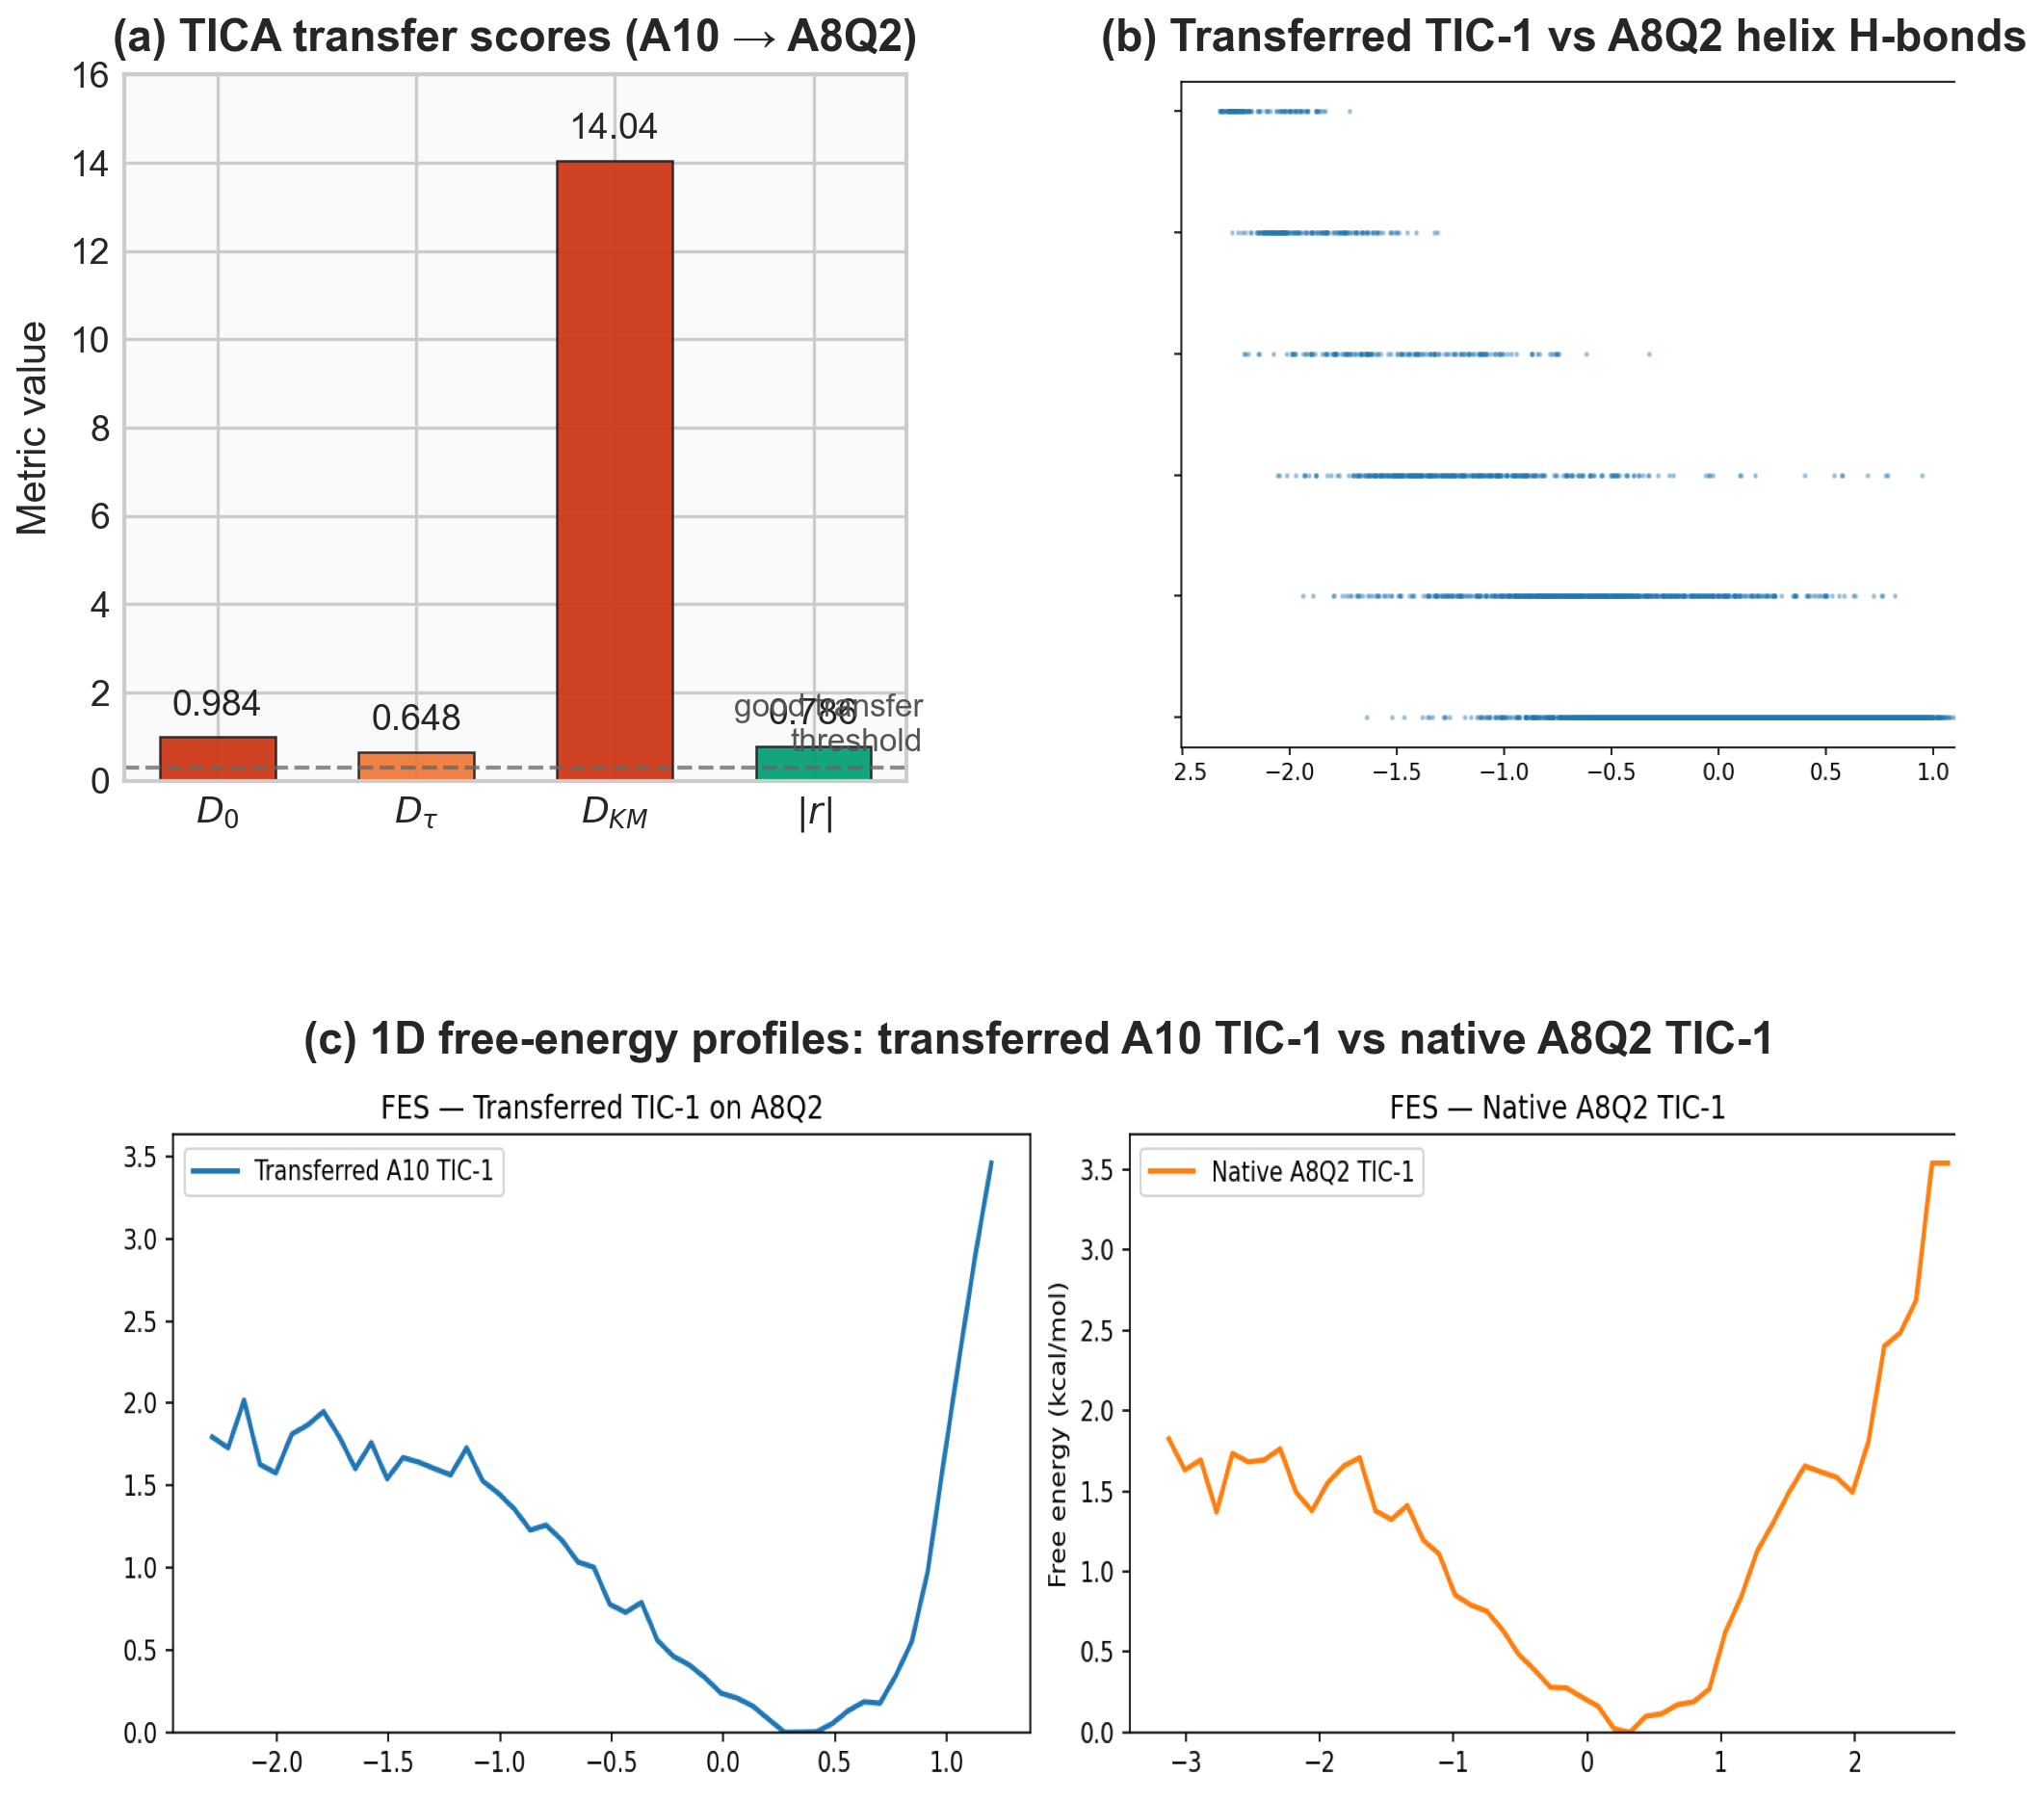
\includegraphics[width=0.95\textwidth]{transfer_diagnostics.png}
    \caption[TICA transfer diagnostics (A10$\to$A8Q2)]{TICA transfer diagnostics from A10 to A8Q2. (a)~Four transfer metrics (axis labels give definitions): $D_0$ and $D_{KM}$ lie in the poor regime relative to the dashed criteria, $D_\tau$ is marginal, and the absolute correlation $|r|$ between transferred TIC-1 and A8Q2 helix content meets the success threshold. The headline is therefore failed global transfer with a retained helix-direction signal. (b)~Scatter plot of transferred TIC-1 versus A8Q2 hydrogen-bond count $N_{\mathrm{HB}}$, confirming the negative correlation: more negative TIC-1 corresponds to higher helicity. (c)~One-dimensional free-energy profiles along the transferred A10 TIC-1 (left, blue) and along native A8Q2 TIC-1 (right, orange), illustrating why the scalar metrics in (a) read as poor transfer even though a useful helix trend remains.}
    \label{fig:transfer}
\end{figure}

\subsection{TICA2D Gives a Low Short-Budget Helix Error}

The clearest $80$\,ns observable result was obtained with TICA2D two-phase acquisition using $T_c=2$\,ns chunks. COMPASS selected 40 chunks and achieved a helix-fraction error of $\epsilon_{\mathrm{helix}}=7.5\times 10^{-4}$, compared with $2.08\times 10^{-2}$ for bootstrap random acquisition, a 28-fold reduction in the absolute deviation from the full-target reference. The open-fraction error also improved, from $\epsilon_{\mathrm{open}}=3.09\times 10^{-2}$ (random) to $2.04\times 10^{-2}$ (COMPASS). Important source-bin coverage was complete for COMPASS (1.000) and essentially complete for random ($0.992$).

This improvement did \emph{not} coincide with better global distributional metrics. The same run had a worse final TICA-space JSD than random ($0.156$ vs.\ $0.139$) and lower raw bin coverage ($0.514$ vs.\ $0.572$). The short-budget result is therefore not a generic ``COMPASS beats random'' claim. It is a targeted result: transferred TICA density guidance recovers a helix-relevant observable under limited budget, while bootstrap random remains stronger for broad target-distribution coverage.
Figure~\ref{fig:tica80} summarizes cumulative metrics versus sampled budget for this configuration.

\begin{figure}[htbp]
    \centering
    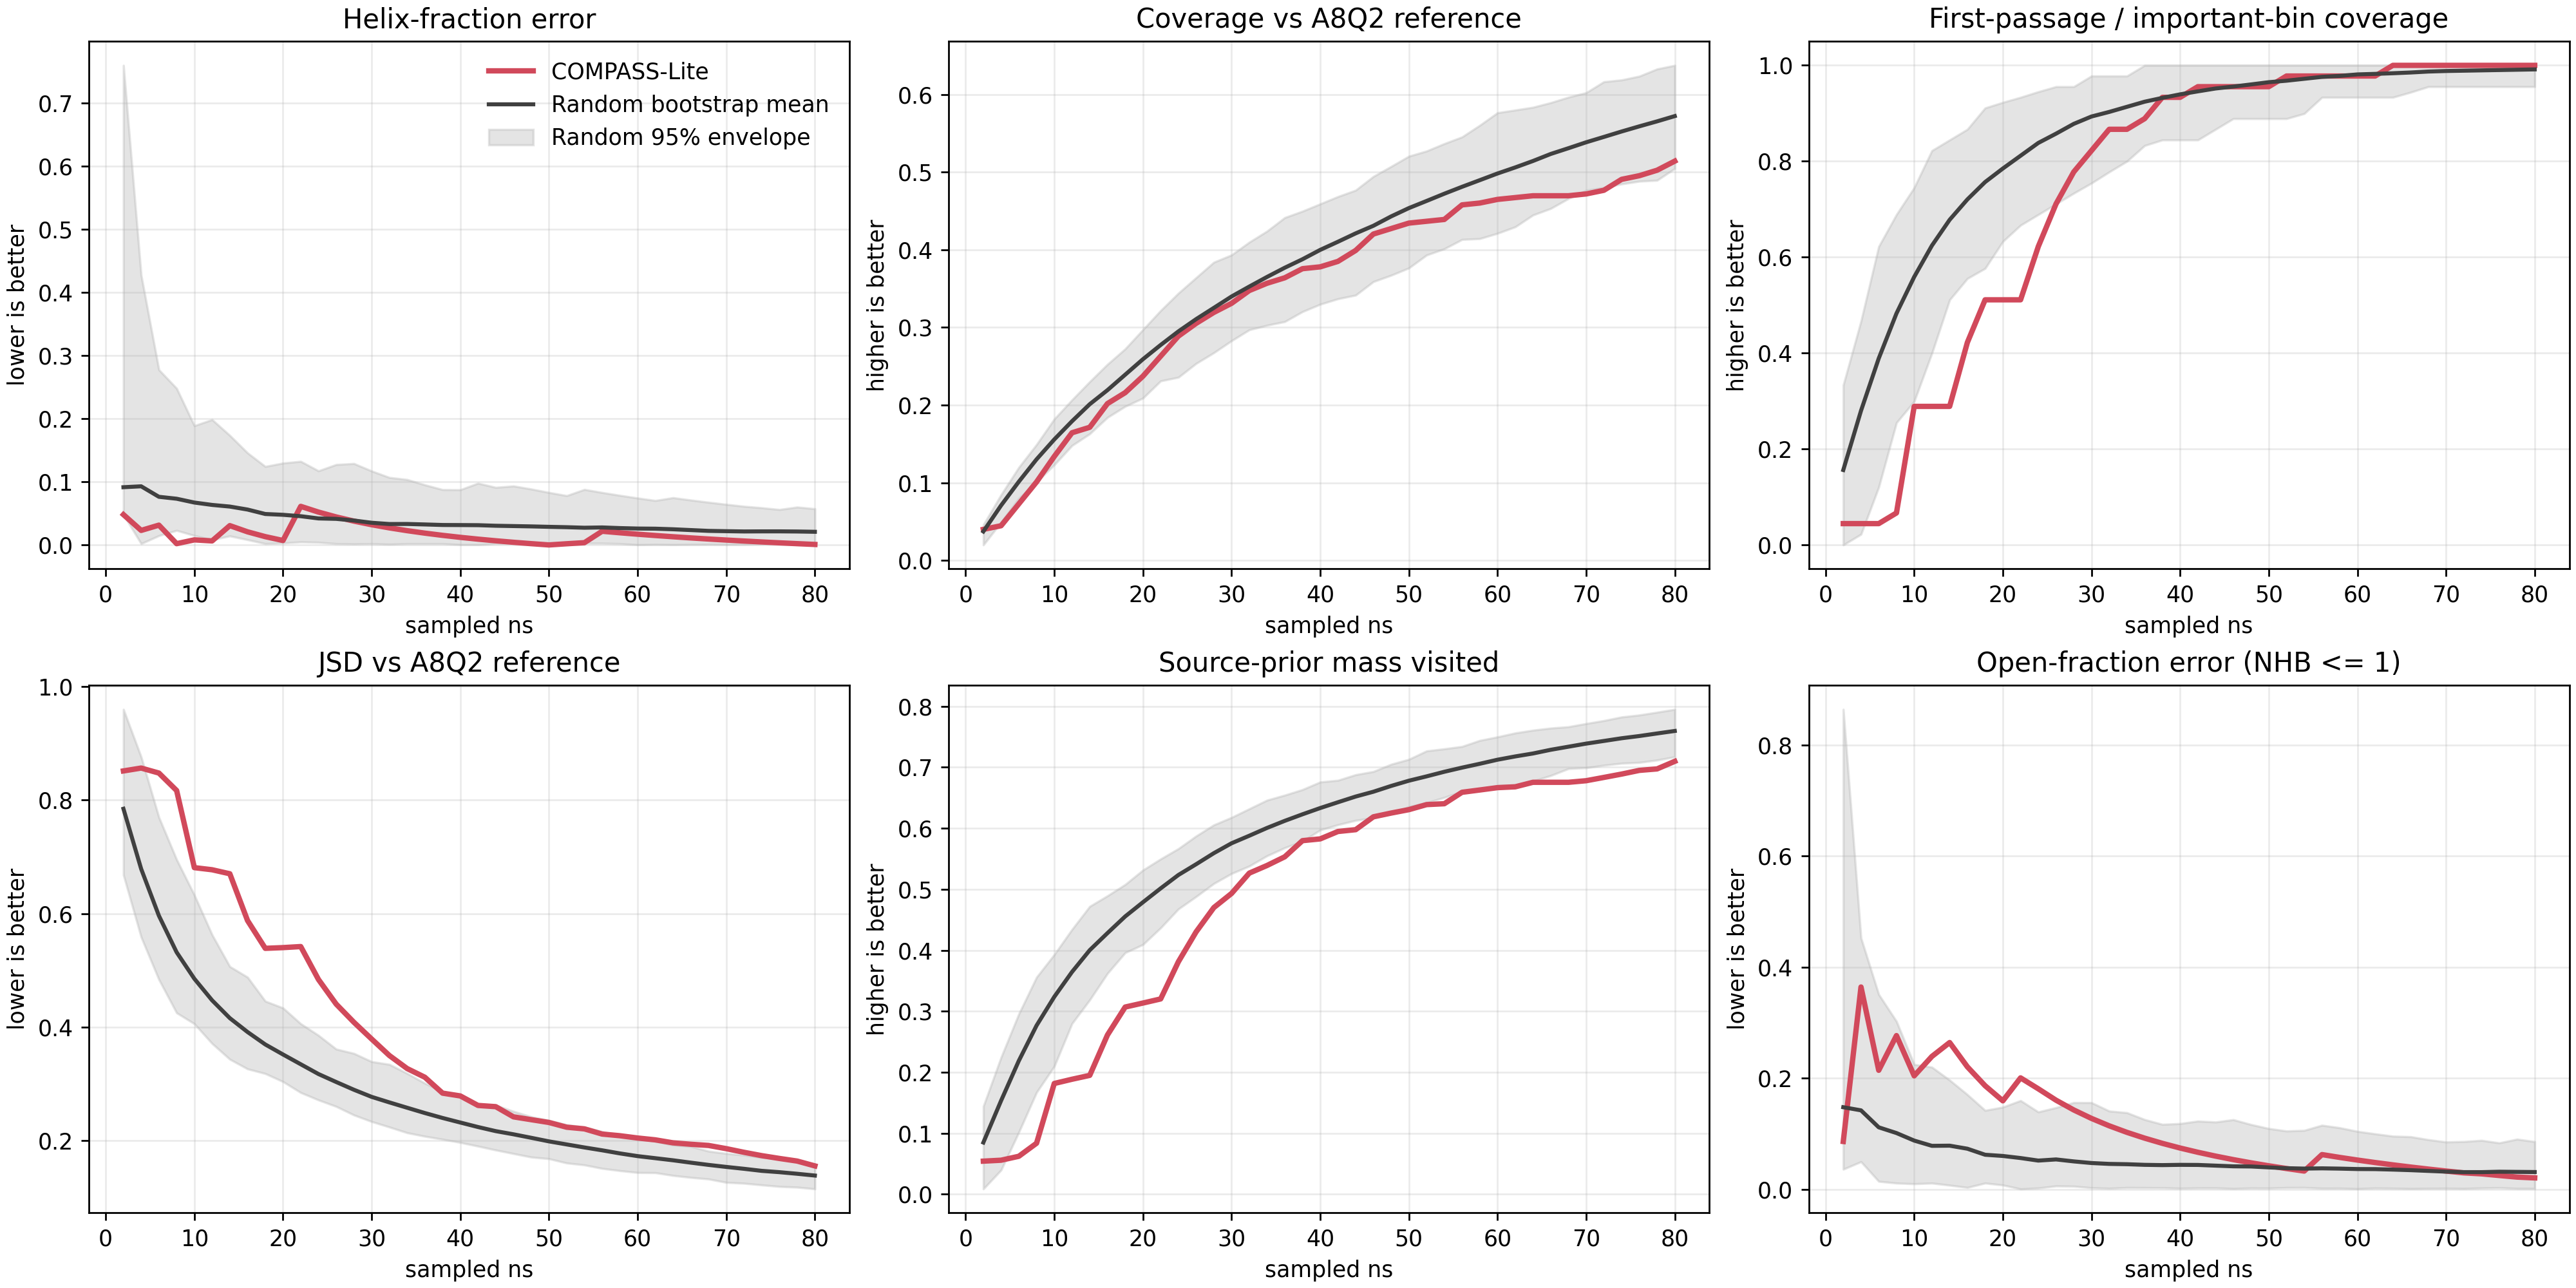
\includegraphics[width=0.95\textwidth]{replay_tica2d_chunk20_80ns.png}
    \caption[Short-budget ($80$\,ns) TICA2D replay vs.\ random]{Short-budget TICA2D acquisition with $T_c=2$\,ns chunks ($80$\,ns total acquired time, 40 chunks). Cumulative metrics versus selected fraction of budget for COMPASS (solid) and bootstrap random (mean $\pm$ shaded band over 100 repeats). Panels show, from top-left to bottom-right: helix-fraction error $\epsilon_{\mathrm{helix}}$, open-fraction error $\epsilon_{\mathrm{open}}$, TICA-space JSD against the full-target reference, and raw bin coverage. COMPASS gives the lowest observed helix-fraction error of any main $80$\,ns experiment in this study, while random remains competitive or better for JSD and raw coverage.}
    \label{fig:tica80}
\end{figure}

\subsection{SPIB1D Accelerates Discovery but Not Equilibrium Estimation}

SPIB1D produced the strongest discovery behavior. At $80$\,ns, SPIB1D two-phase acquisition saturated all three SPIB-space discovery metrics (raw coverage, important-bin coverage, and source-mass visitation all reached $1.000$), compared with random means of $0.863$, $0.963$, and $0.989$ respectively.

The same run, however, performed poorly on helix and open observables. The helix-fraction error was $\epsilon_{\mathrm{helix}}=8.33\times 10^{-2}$ for COMPASS compared with $1.71\times 10^{-2}$ for random, an almost fivefold inflation. The open-fraction error was $7.79\times 10^{-2}$ vs.\ $2.35\times 10^{-2}$ for random. JSD in the SPIB map was also worse than random ($0.014$ vs.\ $0.009$). This cleanly separates two roles that are often conflated in adaptive sampling: a transferred latent coordinate may be excellent for discovering distinct regions while being unsuitable as an equilibrium-density prior.
Figure~\ref{fig:spib80} shows the corresponding SPIB-space curves and bootstrap envelope.

\begin{figure}[htbp]
    \centering
    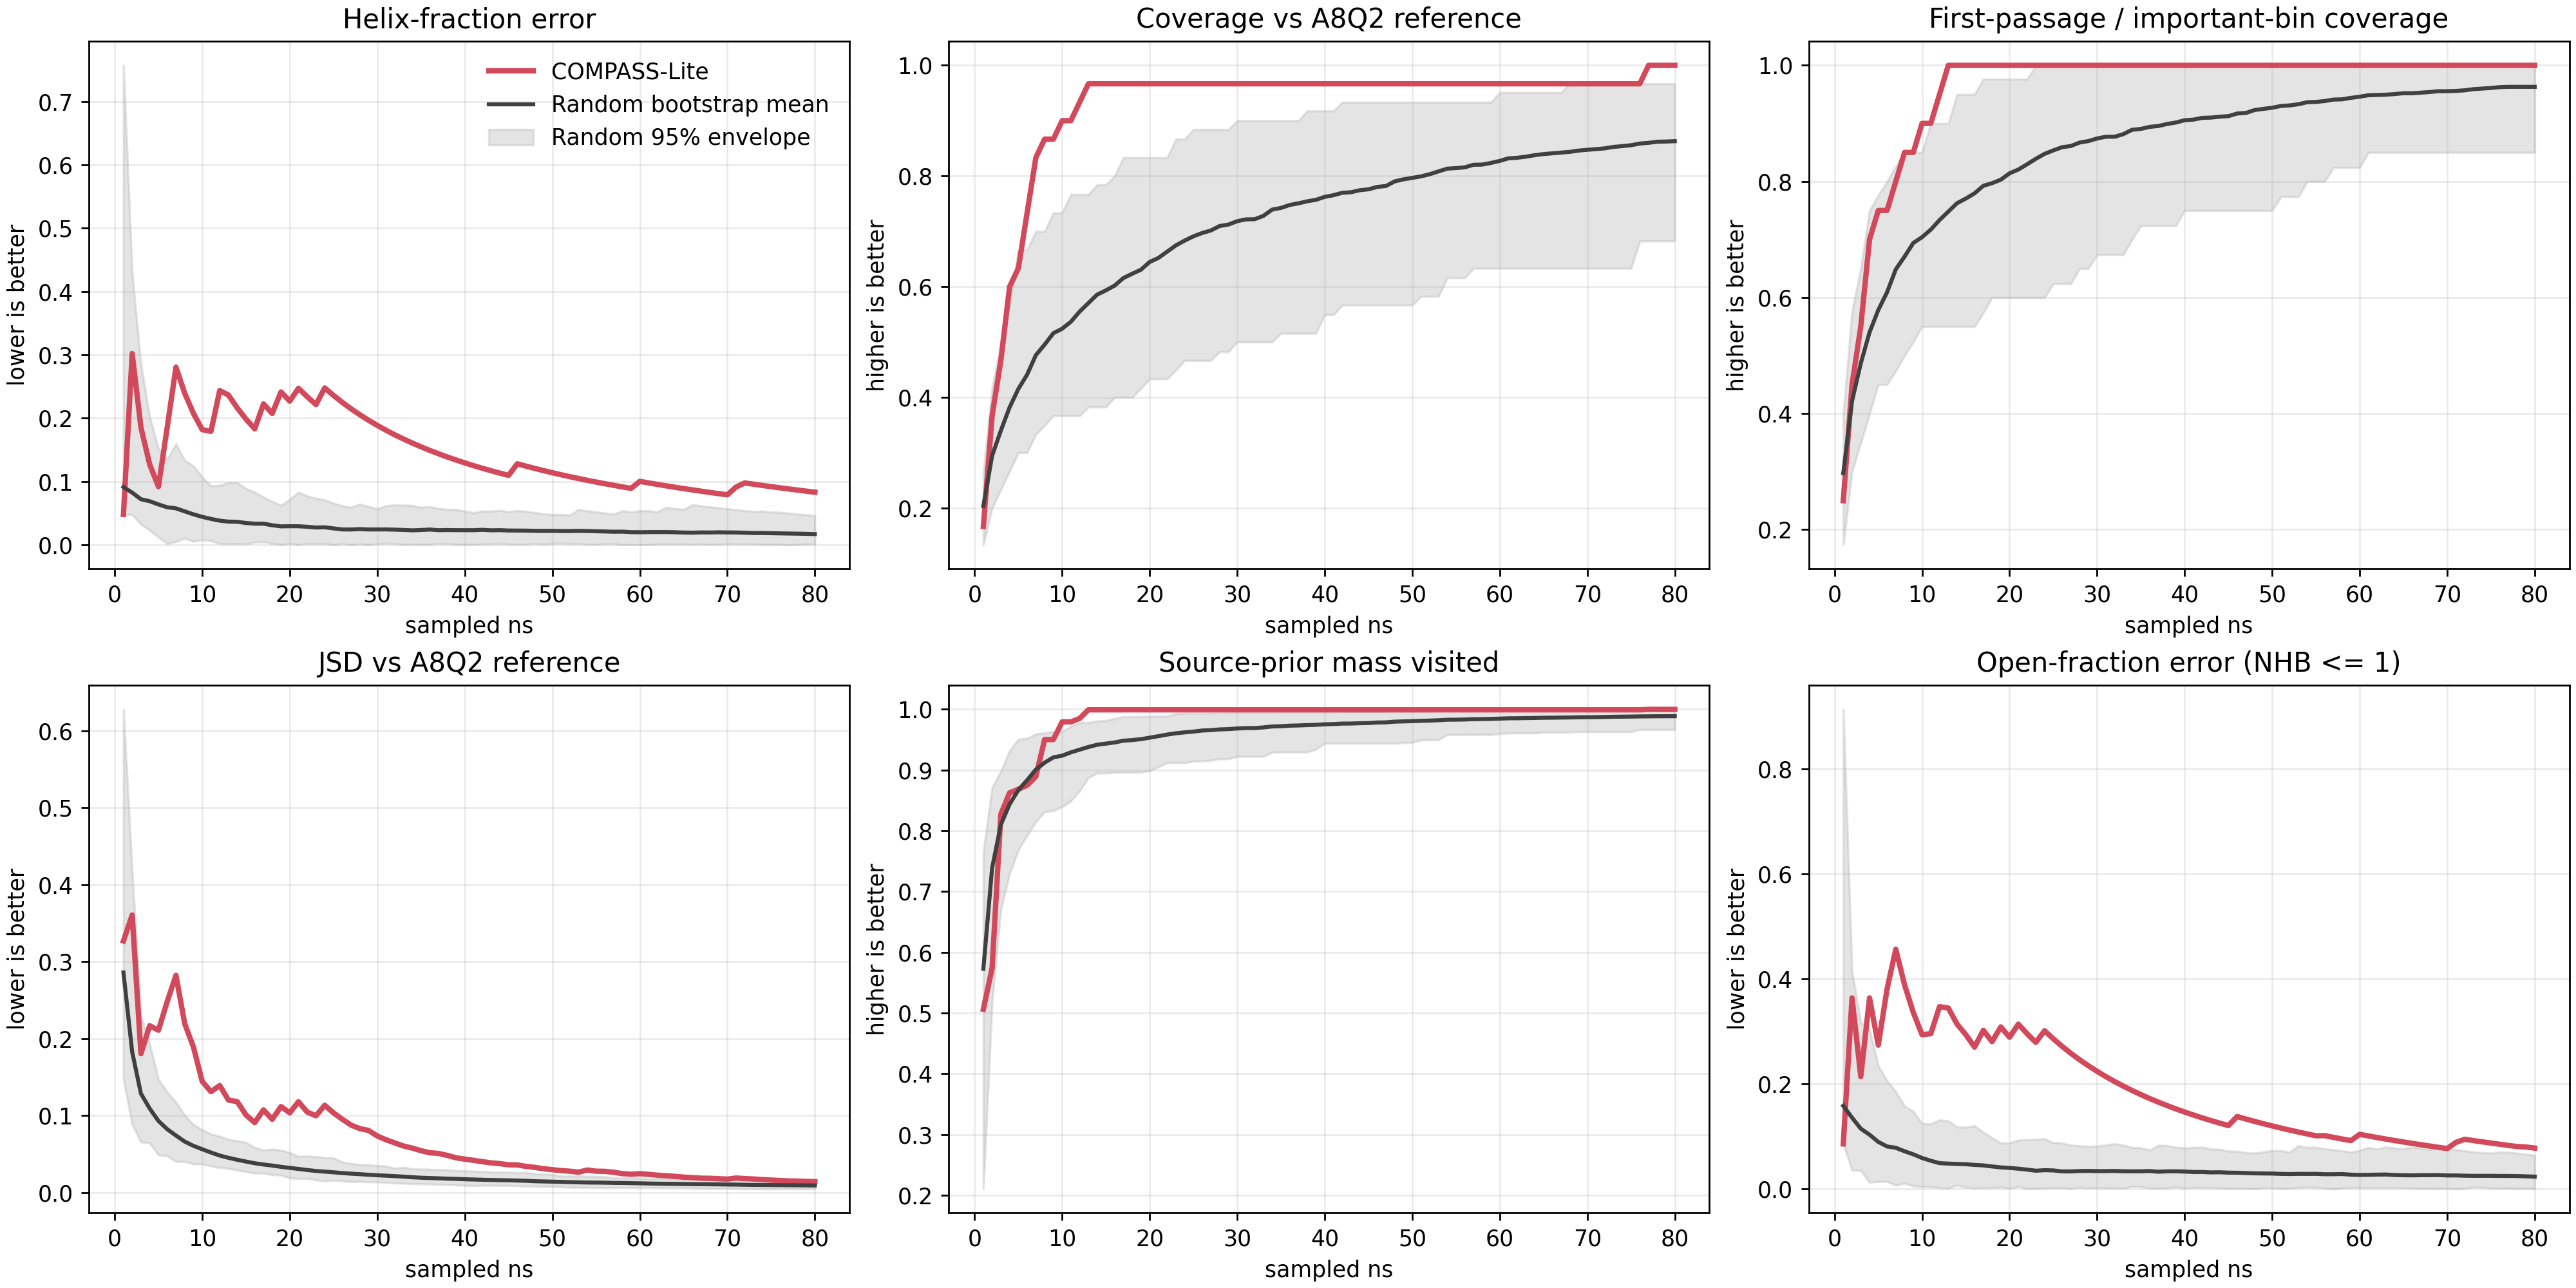
\includegraphics[width=0.95\textwidth]{replay_spib1d_80ns.png}
    \caption[SPIB1D replay ($80$\,ns): coverage vs.\ population metrics]{SPIB1D acquisition at $80$\,ns ($T_c=1$\,ns chunks). Curves and bands as in Fig.~\ref{fig:tica80} but with SPIB-space metrics. SPIB1D rapidly saturates source-supported latent coverage but substantially worsens helix/open population estimates, indicating that the transferred SPIB latent should be treated as a discovery coordinate rather than as a density prior.}
    \label{fig:spib80}
\end{figure}

\subsection{TICA2D Improves Long-Budget Distributional Recovery}

At a $200$\,ns budget, TICA2D two-phase acquisition improved both global JSD and coverage relative to random. COMPASS achieved JSD $0.042$ vs $0.057$ for random, raw coverage $0.880$ vs $0.801$, and source mass visited $0.911$ vs $0.875$. Important-bin coverage was saturated for both policies.

The long-budget result indicates that the short-budget JSD gap versus random seen in Fig.~\ref{fig:tica80} (2\,ns chunks, \SI{80}{ns}) need not persist when acquisition continues on a comparable two-phase TICA policy. Here, longer runs use \SI{1}{ns} chunks (Fig.~\ref{fig:tica200}); qualitatively, early budget still pays for source-deficit repair, whereas later budget lets the density terms repopulate high-mass target bins and improve JSD and coverage relative to bootstrap random.

\begin{figure}[htbp]
    \centering
    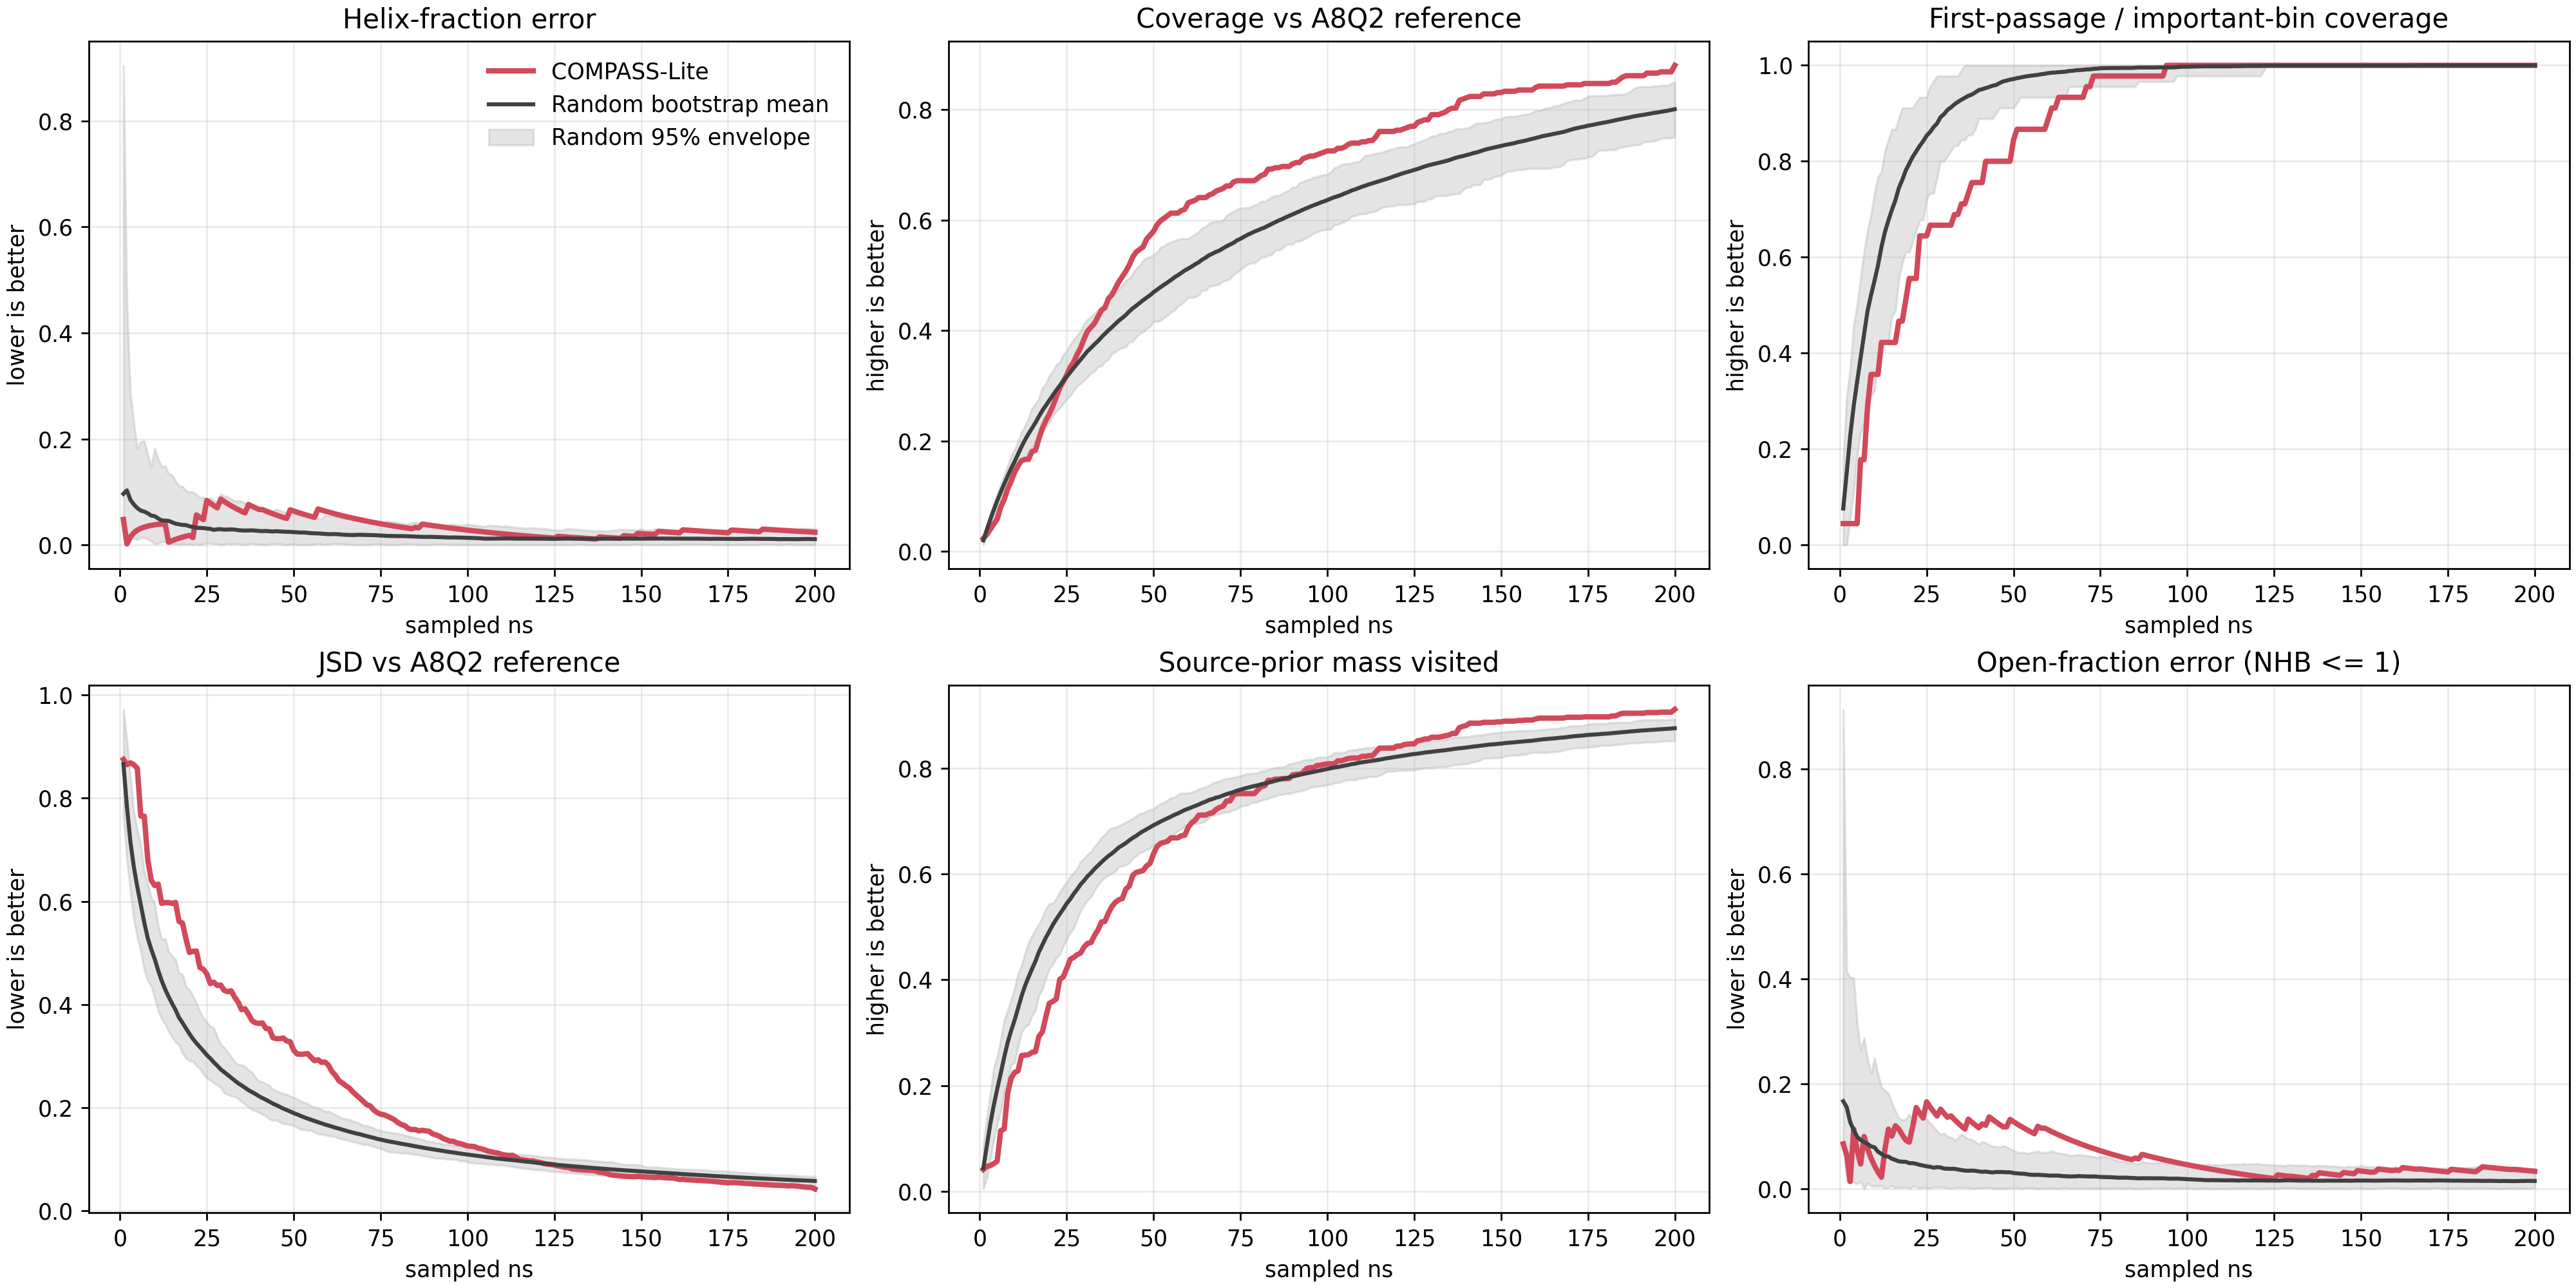
\includegraphics[width=0.95\textwidth]{replay_tica2d_200ns.png}
    \caption[Long-budget ($200$\,ns) TICA2D replay vs.\ random]{Long-budget TICA2D acquisition ($200$\,ns total, $T_c=1$\,ns chunks). Same metric panels as Fig.~\ref{fig:tica80}. At $200$\,ns the TICA2D two-phase policy improves JSD, raw coverage, and source-mass visitation relative to bootstrap random acquisition, showing that the short-budget distributional penalty can be overcome with sufficient budget.}
    \label{fig:tica200}
\end{figure}

\subsection{Prior Quality Controls the Failure Mode}\label{sec:prior_quality}

Deliberately corrupted TICA priors showed that COMPASS follows its prior rather than ignoring it. Key $80$\,ns summary metrics are given in Table~\ref{tab:prior_quality}. A uniform prior increased coverage but degraded JSD and observables. A shuffled prior improved coverage and important coverage but no longer improved distributional accuracy. The inverted prior produced the strongest failure: JSD increased to 0.273 compared with 0.132 for random, and helix/open errors were substantially worse than random. A noisy prior was less damaging and remained closer to random.

\begin{table}[htbp]
    \centering
    \caption{Selected $80$\,ns prior-quality tests for TICA2D two-phase acquisition ($T_c=1$\,ns chunks). \emph{Clean} is the uncorrupted A10 prior. Lower JSD and lower observable errors are better.}
    \label{tab:prior_quality}
    \small
    \setlength{\tabcolsep}{4pt}
    \begin{tabular}{lcccccc}
        \toprule
        Prior & JSD & Random JSD & Coverage & Random coverage & Helix error & Open error \\
        \midrule
        Clean & 0.147 & 0.132 & 0.528 & 0.583 & 0.0045 & 0.0066 \\
        Uniform & 0.200 & 0.132 & 0.765 & 0.583 & 0.0695 & 0.1079 \\
        Shuffled & 0.151 & 0.132 & 0.725 & 0.583 & 0.0208 & 0.0716 \\
        Inverted & 0.273 & 0.132 & 0.725 & 0.583 & 0.0645 & 0.1154 \\
        Noisy & 0.140 & 0.132 & 0.563 & 0.583 & 0.0245 & 0.0216 \\
        \bottomrule
    \end{tabular}
\end{table}

The inverted-prior result is mechanistically useful even though it is a performance failure. It proves that the source prior is active in the policy. It also shows that prior trust cannot be treated as a minor implementation detail: a bad prior can actively steer acquisition toward the wrong target distribution.
Figure~\ref{fig:prior_maps} overlays chunk-selection footprints on the target trajectory for the correct versus inverted prior.

\begin{figure}[htbp]
    \centering
    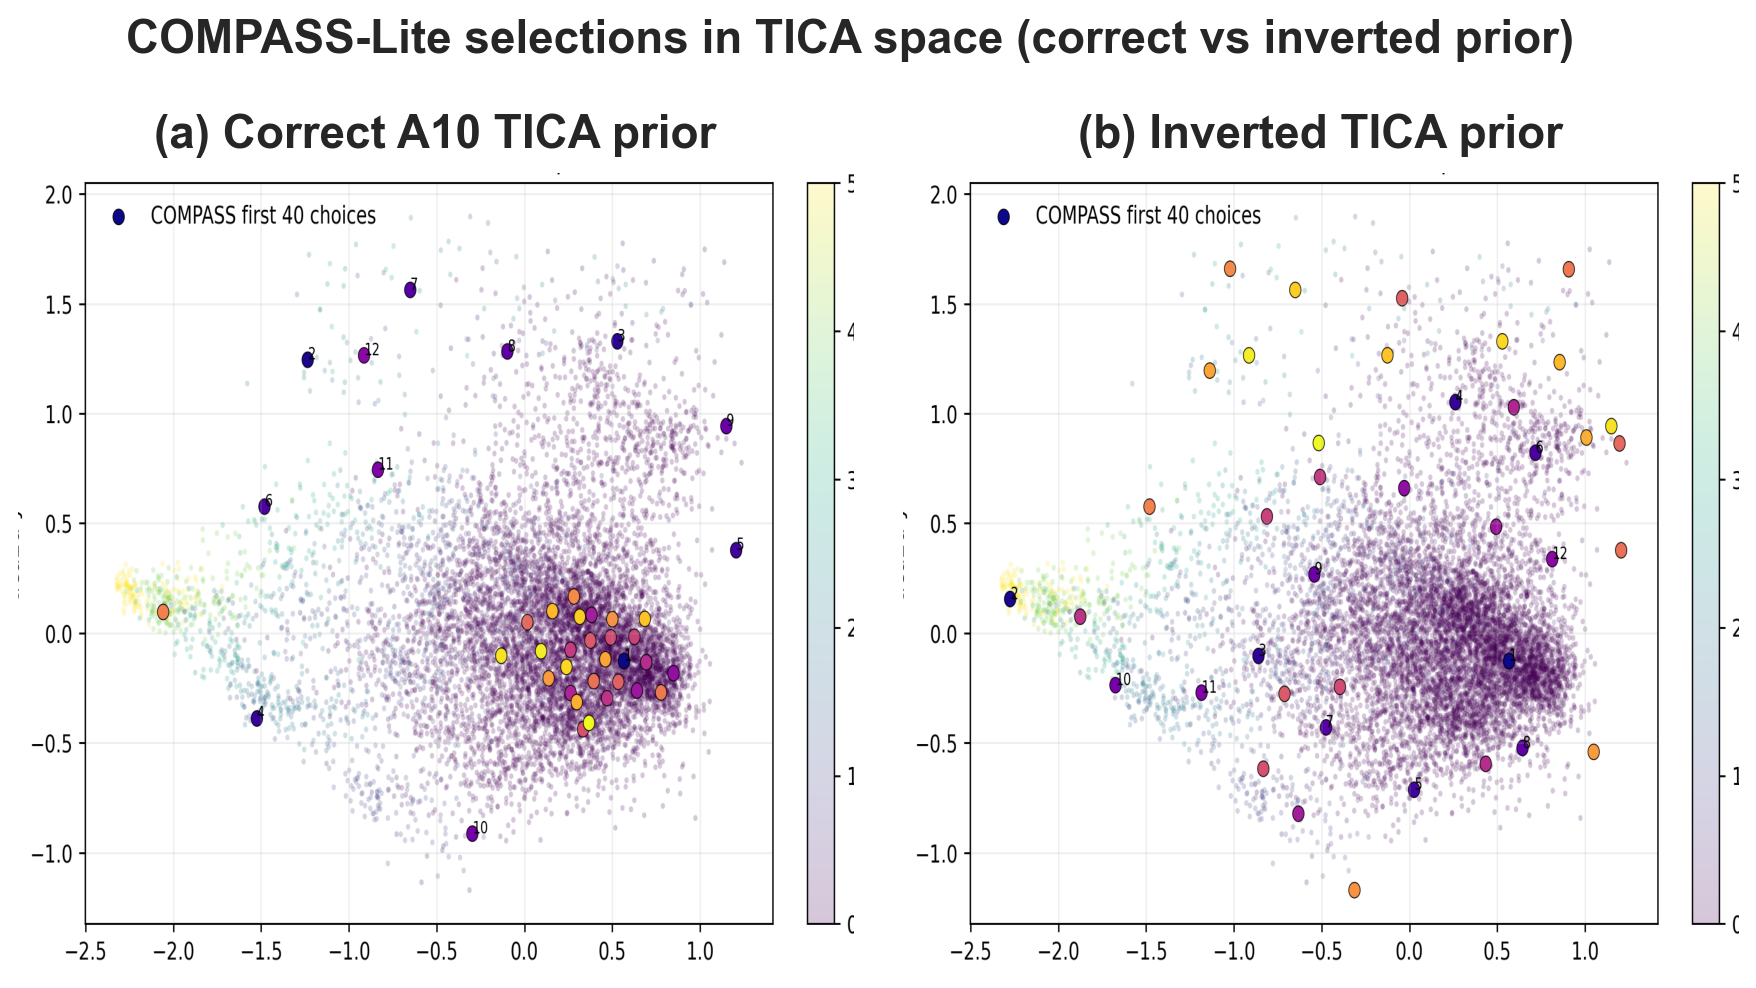
\includegraphics[width=0.95\textwidth]{prior_corruption_probe_maps.png}
    \caption[COMPASS chunk selections: correct vs.\ inverted TICA prior]{COMPASS chunk selections in TICA space under (a)~the correct A10 TICA prior and (b)~the inverted TICA prior. Background points show the A8Q2 target trajectory colored by hydrogen-bond count (yellow = high helix, purple = open); large numbered circles mark the first 40 COMPASS selections. Under the correct prior, selections concentrate in the dense core where most source-supported mass lies. Under the inverted prior, selections scatter into the sparse periphery, visually confirming that the policy follows its prior and that an inverted prior actively steers selection away from the target distribution.}
    \label{fig:prior_maps}
\end{figure}

\subsection{Matched-Dynamics Benchmark Isolates Prior and Adaptivity Contributions}
\label{sec:results_msm}

Under the MSM emulator (Section~\ref{sec:methods_msm}), COMPASS (B6) ties or wins on helix/open errors in every preset at the final budget (50 repeats; Table~\ref{tab:msm_benchmark}; Figs.~\ref{fig:msm_grid}, \ref{fig:msm_pair}, \ref{fig:msm_map}). Repeat-level spreads at the final round are shown in Supporting Information Figure~\ref{fig:si_msm_violins}. On SPIB1D only, the single-walk ceiling B0 achieves the lowest JSD because 1D Markov mixing is unusually fast at this grid resolution; here B0 is only a diagnostic, not a fair online comparator.

Pair-difference curves (Fig.~\ref{fig:msm_pair}) decompose the lift: $B6{-}B3$ (prior vs.\ count-based adaptivity alone) is negative on mean final JSD in all five presets; $B3{-}B1$ (adaptivity vs.\ replicas) is negative on JSD everywhere and usually helps observables, except on SPIB1D where min-count overweights minority helical bins on a coarse 1D lattice. Farthest-point B4 is catastrophic on tICA presets ($|\Delta f_{\mathrm{open}}|\approx 0.33$--$0.48$): geometric novelty drives restarts into peripheral low-mass bins (Fig.~\ref{fig:msm_map}), the emulator analogue of inverted-prior failure (Section~\ref{sec:prior_quality}). On SPIB1D, B3/B4 also inflate helix/open errors versus B6 without a density-aware steering signal.

\begin{table}[htbp]
    \centering
    \caption[MSM emulator: final-budget summary table (selected presets)]{MSM-emulator benchmark: final-budget means across 50 repeats for three representative presets. Lower is better for JSD, $|\Delta f_{\mathrm{helix}}|$, $|\Delta f_{\mathrm{open}}|$; higher is better for coverage. Best entry in each column is \textbf{bold}. B0 is the single-walk diagnostic ceiling under Markov dynamics and is optimistic relative to real MD restart cost. Numerical exports for all five emulator presets are archived under \texttt{outputs/msm\_benchmark/}.}
    \label{tab:msm_benchmark}
    \small
    \setlength{\tabcolsep}{4pt}
    \begin{tabular}{llcccc}
        \toprule
        Preset & Policy & JSD $\downarrow$ & Coverage $\uparrow$ & $|\Delta f_{\mathrm{helix}}|$ $\downarrow$ & $|\Delta f_{\mathrm{open}}|$ $\downarrow$ \\
        \midrule
        \multirow{6}{*}{tICA2D baseline, \SI{160}{ns}} & B0 single-walk & 0.524 & 0.142 & 0.038 & 0.067 \\
        & B1 replicas & 0.618 & 0.106 & 0.044 & 0.080 \\
        & B2 uniform & 0.521 & 0.137 & 0.037 & \textbf{0.043} \\
        & B3 min-count & 0.534 & 0.142 & 0.038 & 0.067 \\
        & B4 farthest & 0.735 & 0.102 & 0.090 & 0.381 \\
        & B6 COMPASS & \textbf{0.509} & 0.142 & \textbf{0.028} & 0.045 \\
        \midrule
        \multirow{6}{*}{SPIB1D, \SI{160}{ns}} & B0 single-walk & \textbf{0.063} & 0.540 & \textbf{0.025} & \textbf{0.031} \\
        & B1 replicas & 0.320 & 0.599 & 0.053 & 0.088 \\
        & B2 uniform & 0.117 & 0.625 & 0.084 & 0.106 \\
        & B3 min-count & 0.213 & \textbf{0.756} & 0.215 & 0.264 \\
        & B4 farthest & 0.319 & 0.725 & 0.247 & 0.286 \\
        & B6 COMPASS & 0.077 & 0.545 & 0.037 & 0.045 \\
        \midrule
        \multirow{6}{*}{tICA2D long, \SI{400}{ns}} & B0 single-walk & 0.334 & 0.285 & 0.024 & 0.039 \\
        & B1 replicas & 0.555 & 0.156 & 0.045 & 0.081 \\
        & B2 uniform & 0.359 & 0.270 & 0.031 & 0.034 \\
        & B3 min-count & 0.374 & \textbf{0.290} & 0.036 & 0.106 \\
        & B4 farthest & 0.646 & 0.202 & 0.040 & 0.479 \\
        & B6 COMPASS & \textbf{0.316} & 0.277 & \textbf{0.019} & \textbf{0.031} \\
        \bottomrule
    \end{tabular}
\end{table}

\begin{figure}[htbp]
    \centering
    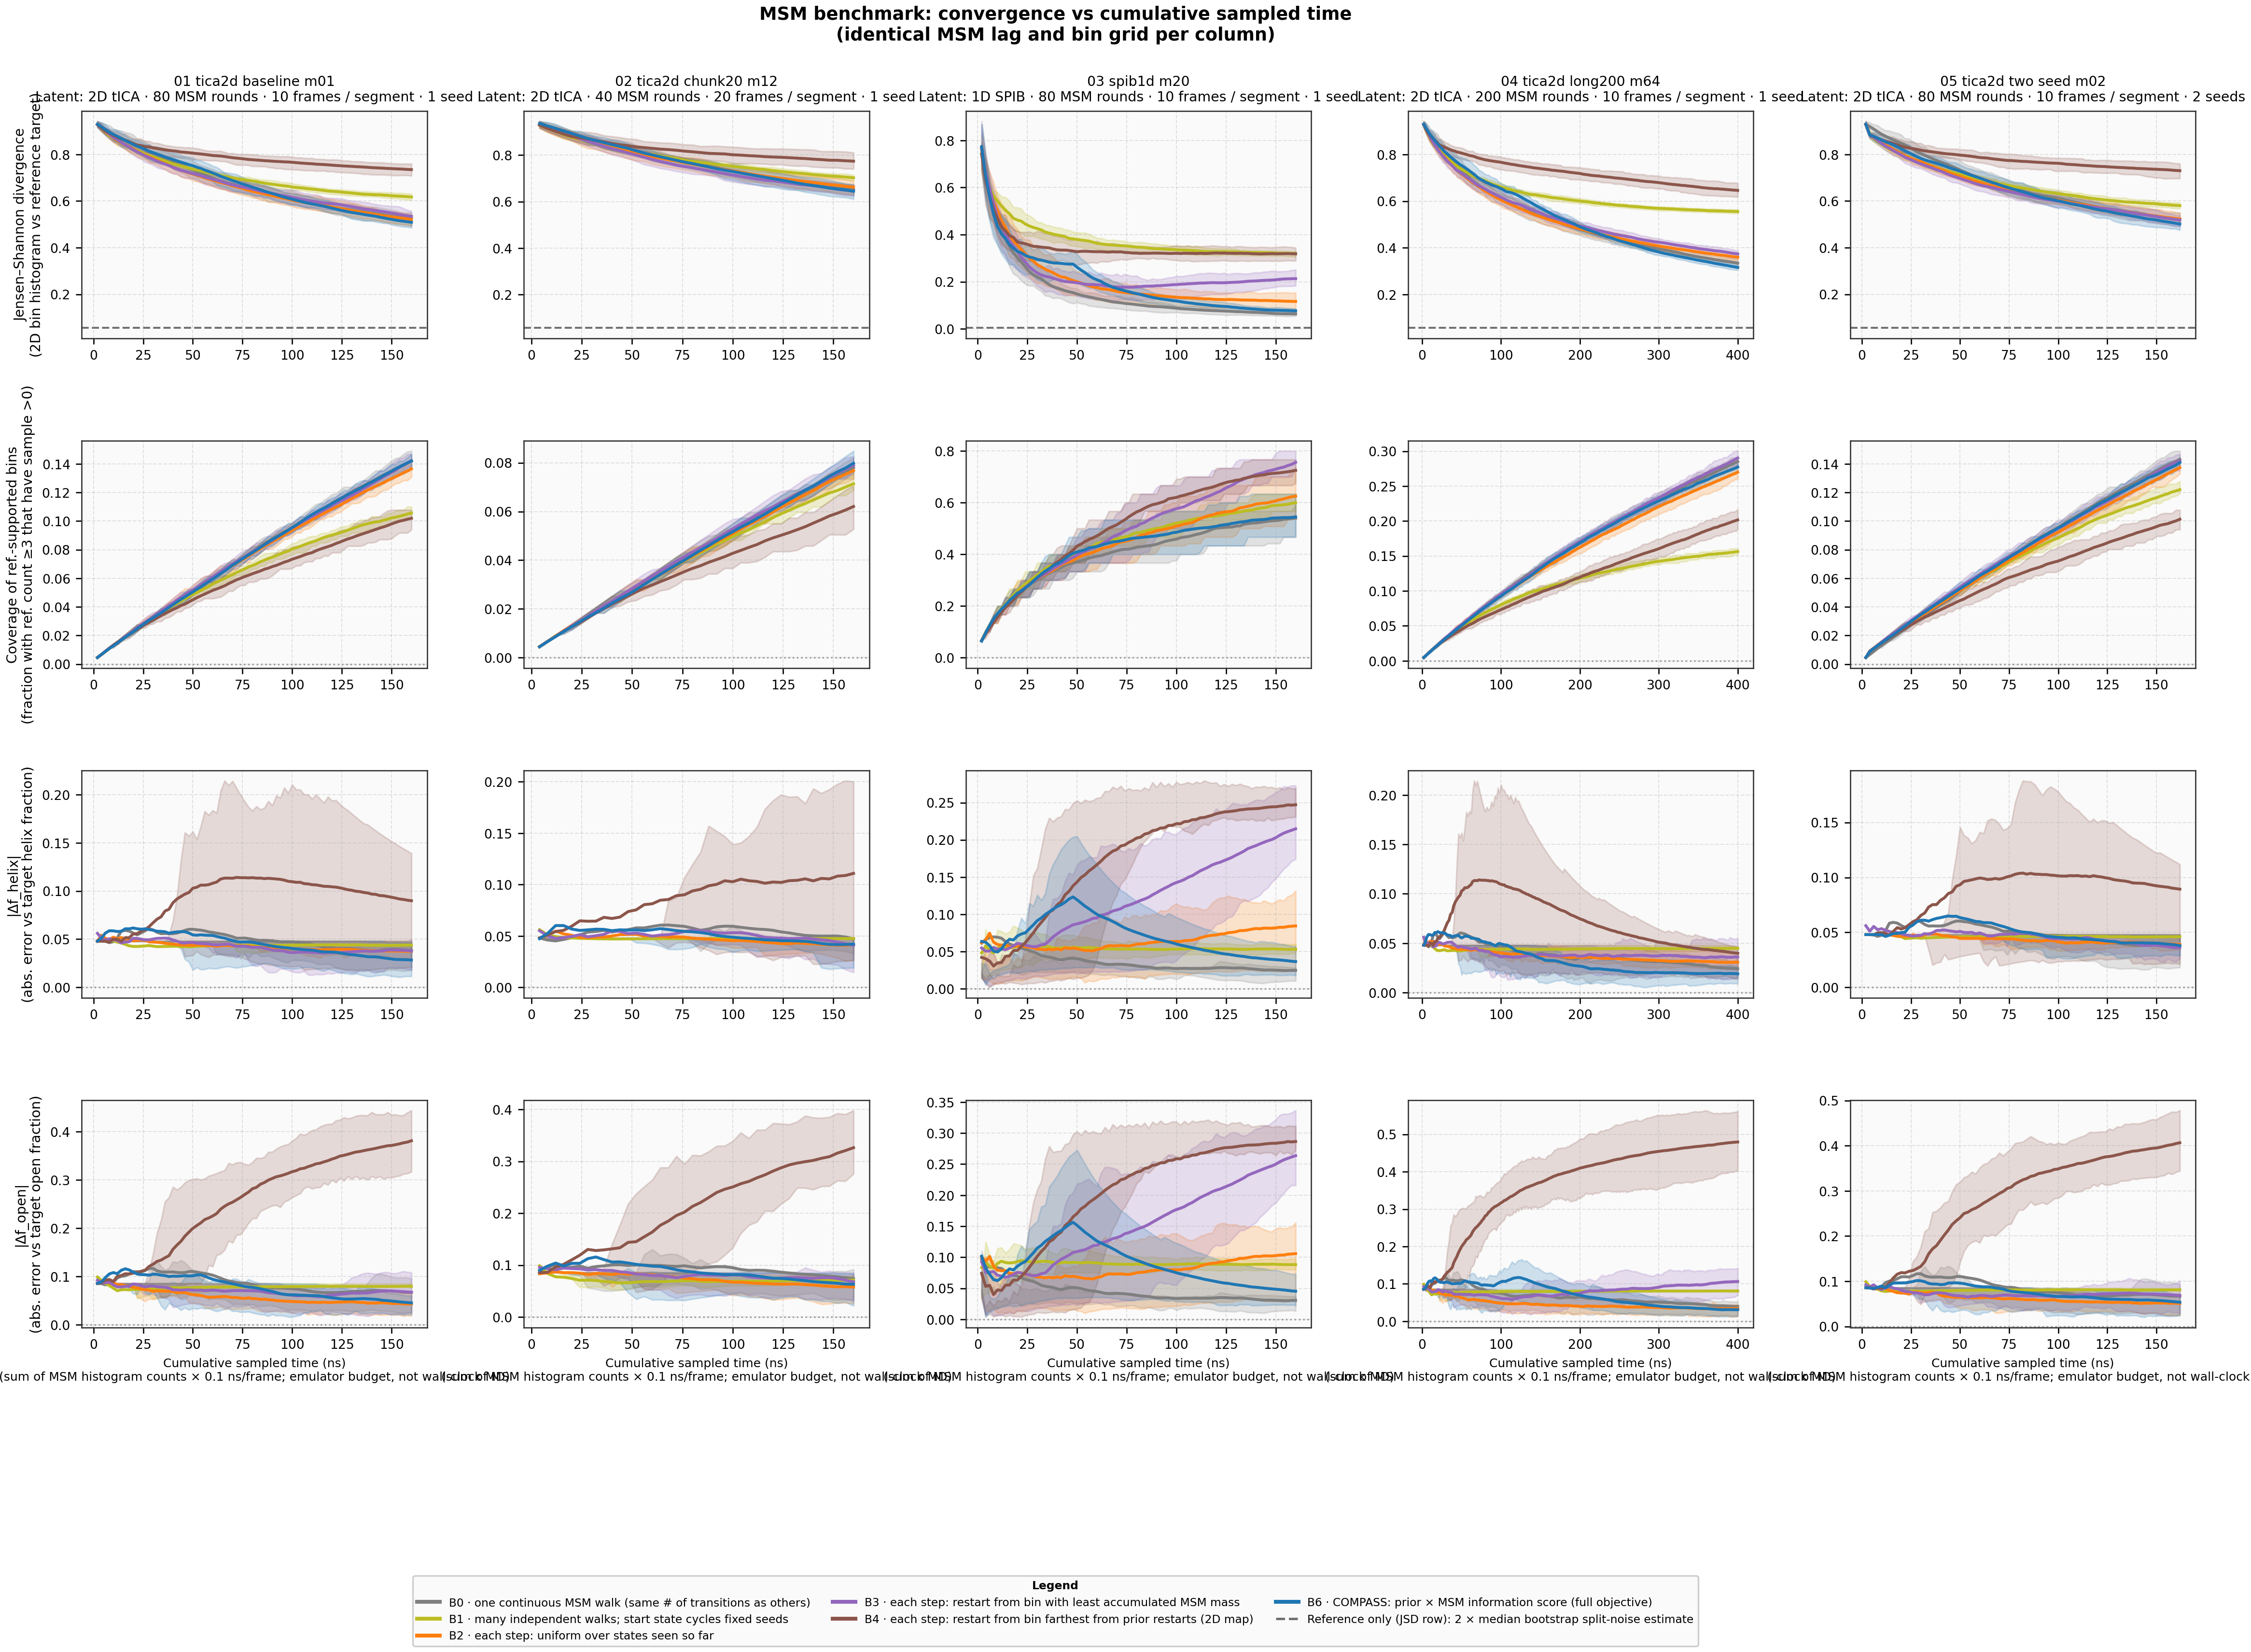
\includegraphics[width=0.98\textwidth]{msm_convergence_grid.png}
    \caption[MSM emulator: convergence curves across presets]{MSM-emulator benchmark: convergence of four metrics (rows: JSD, coverage of reference-supported bins, $|\Delta f_{\mathrm{helix}}|$, $|\Delta f_{\mathrm{open}}|$) versus lag-weighted cumulative sampled time (ns), across five preset configurations (columns). Lines show means; shaded bands show the interquartile range across 50 independent repeats. Horizontal dashed line on the JSD row is twice the median bootstrap split-noise estimate for that preset. Across every preset, COMPASS (B6, blue) matches or beats count-based min-count (B3, purple) and independent replicas (B1, olive) on the two observable errors, while farthest-point exploration (B4, brown) diverges on $|\Delta f_{\mathrm{open}}|$ in all tICA presets.}
    \label{fig:msm_grid}
\end{figure}

\begin{figure}[htbp]
    \centering
    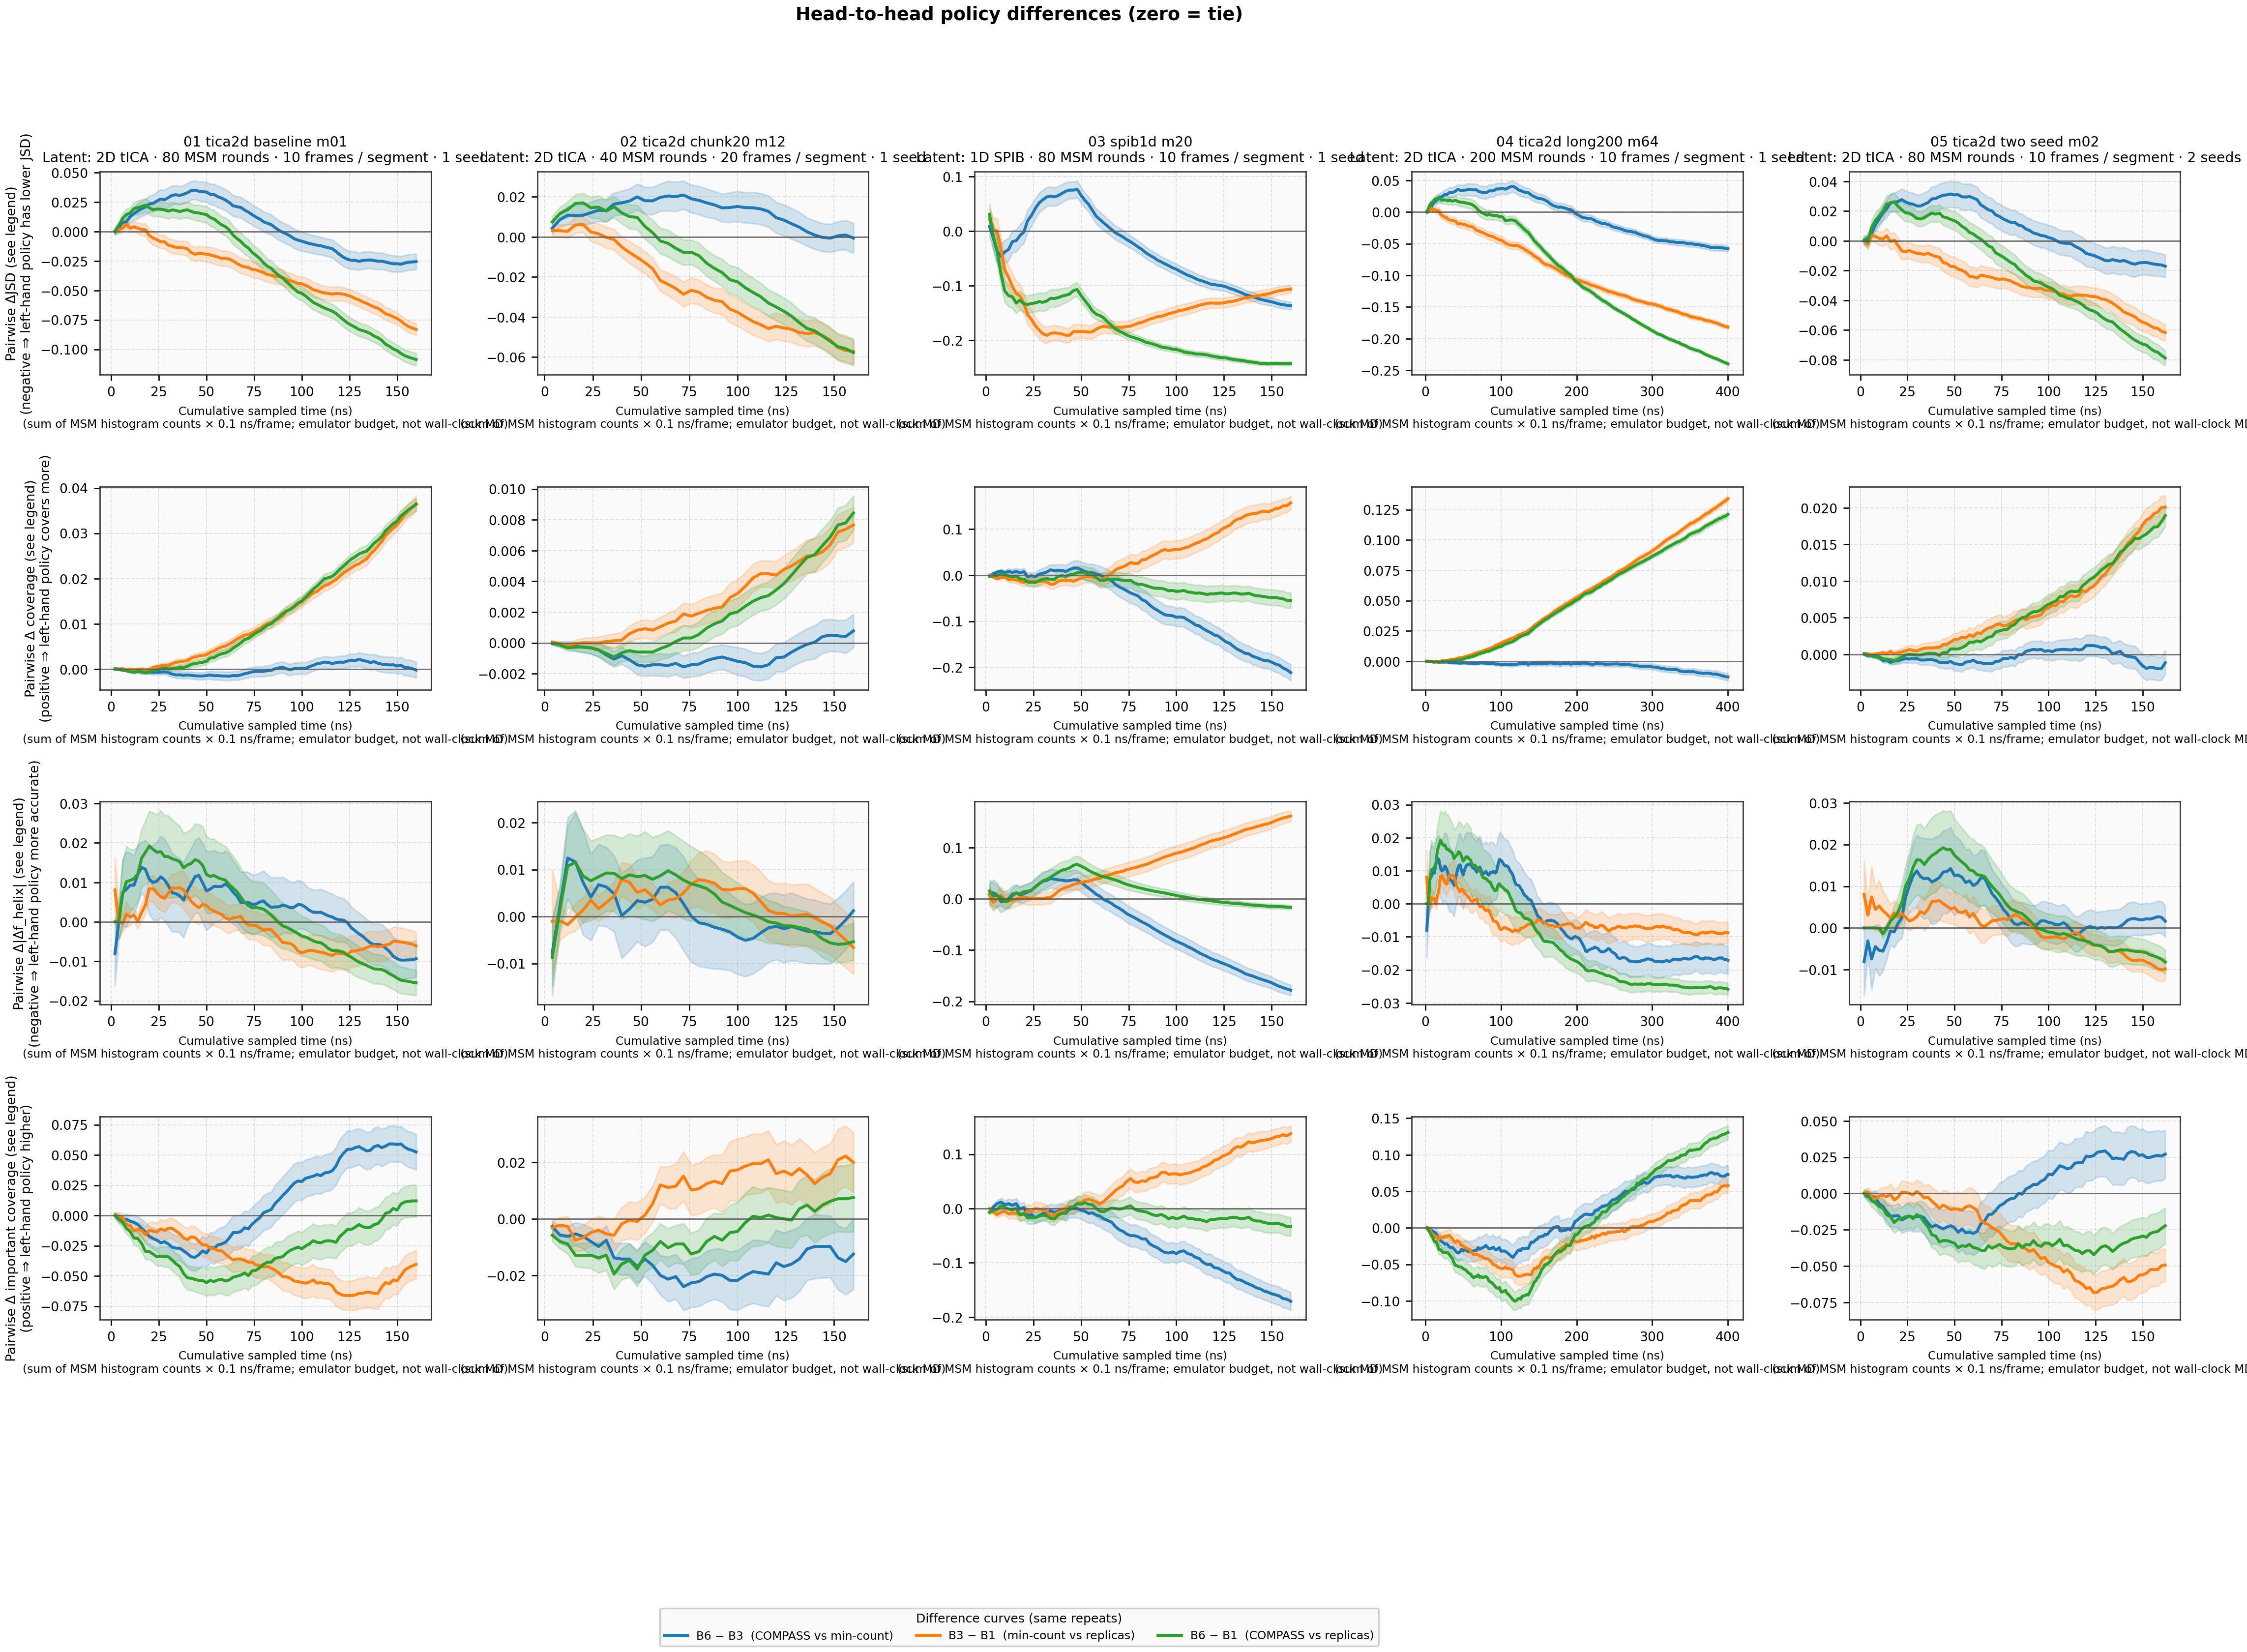
\includegraphics[width=0.98\textwidth]{msm_pair_delta_curves.png}
    \caption[MSM emulator: $B6{-}B3$, $B3{-}B1$, and $B6{-}B1$ pair differences]{Head-to-head pair differences along the same random repeats of Fig.~\ref{fig:msm_grid}: $B6-B3$ (COMPASS minus min-count, isolating the \emph{prior contribution}), $B3-B1$ (min-count minus replicas, isolating the \emph{adaptivity contribution}), and $B6-B1$ (total lift). For JSD and $|\Delta f_{\mathrm{helix}}|$ a negative value favors the first-named policy; for coverage-like metrics the sign flips (see panel titles). Mean $B6-B3$ on JSD is negative in every preset. The two contributions compound on average: COMPASS tracks the reference more closely than either count-based adaptive sampling alone or non-adaptive replicas alone.}
    \label{fig:msm_pair}
\end{figure}

\begin{figure}[htbp]
    \centering
    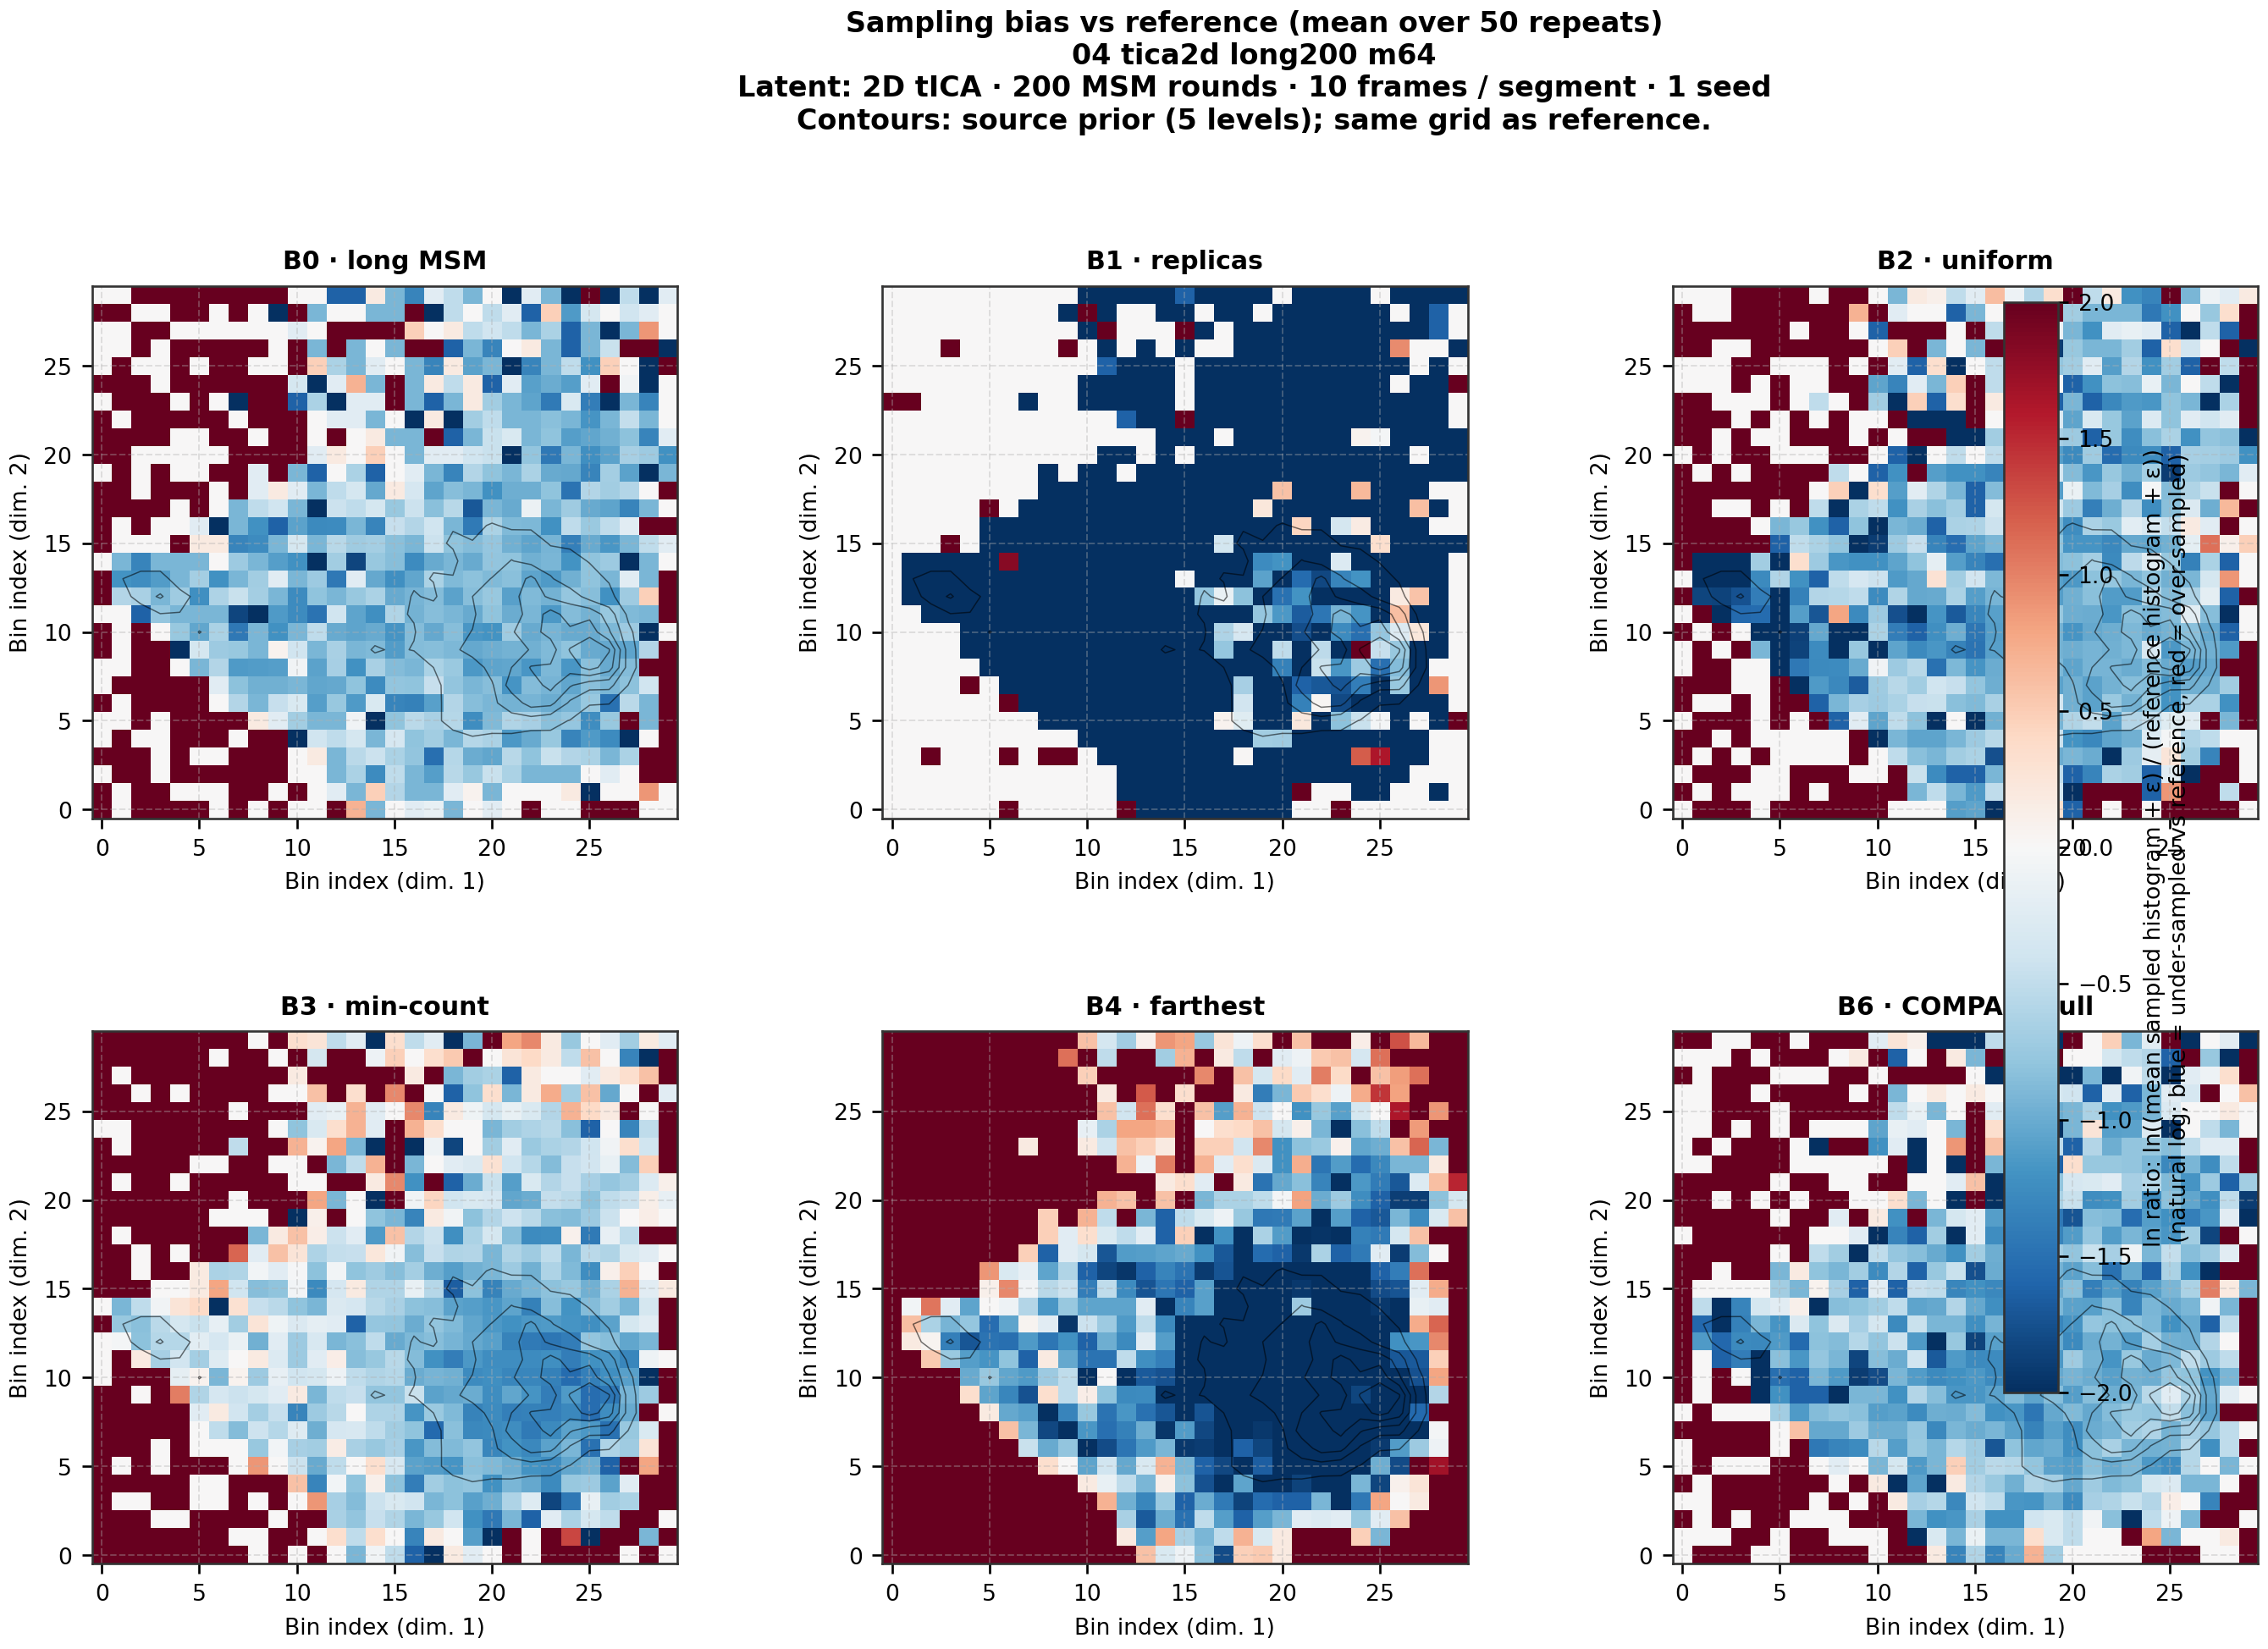
\includegraphics[width=0.98\textwidth]{msm_map_overlay_tica2d_long400ns.png}
    \caption[MSM emulator: spatial log-ratio maps (long 2D tICA preset)]{MSM-emulator spatial view for the long-budget 2D tICA preset (400\,ns sampled time; same bins and reference as Table~\ref{tab:msm_benchmark}, long row). Each panel averages the final lag-weighted histogram over 50 repeats for the labeled policy and displays $\ln[(\mathrm{mean\ sampled\ mass}+\varepsilon)/(\mathrm{reference\ mass}+\varepsilon)]$ per bin (red: over-sampled vs.\ reference; blue: under-sampled). Black contours trace the source prior. Farthest-point restarts (B4) push mass toward the map periphery; COMPASS (B6) stays nearer the reference core. Raster labels from the plotting script may not match this report's figure numbering.}
    \label{fig:msm_map}
\end{figure}

\section{Discussion}
\label{sec:disc_msm}

\paragraph{Interpretation.}
Transferred TICA remains useful as a \emph{density} and helix-level signal even when global transfer diagnostics are weak; transferred SPIB behaves as a \emph{discovery} coordinate and can corrupt equilibrium observables if treated like a density prior.
No single metric defines success: coverage can increase while observables worsen (Table~\ref{tab:prior_quality}, uniform prior).

\paragraph{Related work.}
Adaptive MD couples exploration and exploitation in learned coordinates.\cite{shamsi2018reap,yang2024werl,leung2025dlwe,perezhernandez2013tica,wang2021spib}
Unlike weighted ensembles,\cite{huber1996we,zuckerman2017weighted} COMPASS does not maintain unbiased trajectory weights or guaranteed kinetic estimates; it is intended as an \emph{evaluation-first} construction---a transparent staging test for whether a proposed prior would steer acquisition productively before committing to expensive online simulations.
Retrospective replay isolates prior behavior on a fixed library and does not demonstrate wall-clock acceleration. The MSM emulator complements this by comparing restart \emph{rules} under identical dynamics (Section~\ref{sec:results_msm}); the single-walk baseline $B0$ is optimistic, and two-dimensional MSM grids cannot resolve slow modes outside the bin basis (Section~\ref{sec:tica_atlas}).

\paragraph{Baselines and trust.}
Because bootstrap random sampling draws from the same completed library, gains over random are informative but \emph{metric-specific}.
Prior-corruption experiments show that trust in the prior matters more than latent novelty alone (Table~\ref{tab:prior_quality}); hybrid schedules should gate frontier-heavy exploration using measured density-side progress.

\paragraph{Scope.}
Results use a precomputed chunk library (oracle access); SPIB encoders were not fine-tuned on A8Q2; generalization beyond this single A10$\rightarrow$A8Q2 peptide pair remains open.

\chapter{Summary and Conclusions}\label{chap:conclusions}

\section{Summary}

COMPASS is a prior-aware sequential acquisition policy evaluated here on the A10-to-A8Q2 peptide benchmark using retrospective replay and a matched MSM emulator. Evaluation shows whether transferred latent priors are useful for adaptive molecular acquisition in controlled settings. TICA2D guidance yields the most useful density and observable prior for the configurations studied: improved short-budget helix estimation with \SI{2}{ns} chunks and improved JSD and coverage at \SI{200}{ns}. SPIB1D accelerates discovery of source-supported regions but should not be interpreted as an equilibrium-density estimator under transferred encoders. Prior-corruption experiments show that trust calibration, not raw novelty, governs failure modes. The matched-dynamics MSM-emulator benchmark, across five presets and 50 repeats each, separates prior-driven scoring from generic adaptive restarts: COMPASS consistently matches or improves observable errors relative to count-based and replica baselines under identical dynamics, while farthest-point geometric novelty can catastrophically distort observables.

\section{Concluding Remarks}

Retrospective replay (oracle access to all library chunks) and the MSM emulator (restarts only from visited microstates) stress-test complementary aspects of the COMPASS acquisition strategy under prior-guided restarts; together they motivate reading gains against random and against adaptive baselines in context.
The practical lesson is to calibrate trust in transferred priors: exploration without density alignment recurs as the dominant failure mode in both stages.
Future work includes launching new MD from scored states, testing additional mutations and systems, and hybrid controllers that explicitly balance density correction against frontier discovery.


% === Appendix: supporting material included in this PDF
\appendix
\setcounter{table}{0}
\setcounter{figure}{0}
\renewcommand{\thetable}{S\arabic{table}}
\renewcommand{\thefigure}{S\arabic{figure}}
\phantomsection
\part*{Supporting Information}
\label{part:supporting}
\addcontentsline{toc}{part}{Supporting Information}

% Supporting Information body (from COMPASS_JCTC_SUPPORTING_INFORMATION.tex).
% Included in ``paper/COMPASS_BTP_REPORT.tex`` after \appendix; table/figure numbering S-prefix set in main file.

\chapter{Molecular dynamics protocol (source and target trajectories)}

Production trajectories for the wild-type alanine-rich peptide A10 (Ace-(Ala)$_{10}$-NMe) and the mutant A8Q2 (Ace-(Ala)$_8$(Gln)$_2$-NMe) were generated with \textsc{OpenMM}~8.x.\cite{eastman2024openmm8}
We used the additive CHARMM36m protein force field with CHARMM-modified TIP3P water as distributed with \textsc{OpenMM} (\path{charmm36_2024.xml} and matching water parameters).\cite{huang2017charmm36m,kim2015charmmgui}
Nonbonded interactions used a nominal 1.2~nm cutoff with smoothing from 1.0~nm, particle-mesh Ewald electrostatics, constraints on bonds to hydrogen, and rigid water.
Integration used a Langevin middle integrator with 2~fs timestep and friction 1~ps$^{-1}$.
Each system was energy-minimized, equilibrated (NVT with peptide heavy-atom restraints followed by NPT), and simulated in the NVT ensemble for production at \textbf{330~K} to accelerate helix--coil sampling relative to room temperature while preserving the qualitative physics relevant to this benchmark.
The same protocol and temperature were used for A10 and A8Q2 so relative comparisons are internally consistent.

Peptides were solvated in a periodic cubic box with roughly 1.2--1.5~nm buffer and 0.15~M NaCl (see project \path{docs/EXPERIMENT_PROTOCOL.md} for box and ion counts).
Production coordinates were saved at \textbf{0.1~ns} (100~ps) spacing for downstream featurization, consistent with the chunk library described in the main text.
The full A8Q2 trajectory was partitioned into non-overlapping chunks for COMPASS replay; reference observables $f_{\mathrm{helix}}^{\mathrm{ref}}$ and $f_{\mathrm{open}}^{\mathrm{ref}}$ were computed from the same full trajectory.

\chapter{TICA and SPIB training details}

TICA was fit on backbone $\phi/\psi$ (and related) torsional features from the A10 source trajectory using PyEMMA's symmetric time-lagged covariance estimator at a lag matched to the implementation used for production analysis (order 1--4~ns in frame units; see repository \path{src/} and phase-5 analysis logs).
SPIB encoders were trained in PyTorch on the same A10 feature pipeline as in the main experiments, with latent dimension one or two and information-bottleneck trade-off as reported in the main text.

\chapter{Benchmark design and output structure}

The archive-replay benchmark uses pre-recorded A8Q2 trajectory chunks as a library; no new MD is
run during benchmarking.
Chunk scoring and policy dispatch are implemented in \path{src/compass/v2/bench.py}.
The experiment orchestration script \path{scripts/run_experiment_suite.py} resolves caching
dependencies (P1/P2/P3 are CV-agnostic; P2/P3/P4 are noise-agnostic) and dispatches runs via
\texttt{multiprocessing.Pool}.
Reference quantities ($\pi_{\mathrm{ref}}$, per-bin helix fraction, helix--coil boundary TIC-1
value) are precomputed once from the full A8Q2 trajectory by
\path{scripts/precompute_reference.py} and stored under \path{outputs/v2/reference/}.

Output paths follow the convention:
\begin{verbatim}
outputs/v2/experiments/p_{policy}/cv_{cv}/chunk_{c}ns/noise_{n}/repeat_{rr}/
\end{verbatim}
Each \path{v2\_metrics.csv} records per-step: cumulative budget (ns), reweighted helix-fraction
error, reweighted open-fraction error, JSD of the 2D free-energy surface, target-space coverage,
source-space coverage, and cumulative helix$\leftrightarrow$coil transitions.

\chapter{Extended theory, schedule, and supplementary figures}

\subsection*{TICA and SPIB constructions}

Time-lagged independent component analysis seeks coordinates $\boldsymbol\chi(\mathbf{x})$ that maximize autocorrelation at lag $\tau$.\cite{perezhernandez2013tica,schwantes2013improvements}
For mean-free featurized configurations $\mathbf{x}_t$, the instantaneous and symmetric time-lagged covariance matrices are
\begin{equation}
\begin{split}
    \mathbf{C}(0) &= \mathbb{E}_t\!\left[\mathbf{x}_t \mathbf{x}_t^{\top}\right],\\
    \mathbf{C}(\tau) &= \tfrac{1}{2}\mathbb{E}_t\!\left[\mathbf{x}_t \mathbf{x}_{t+\tau}^{\top} + \mathbf{x}_{t+\tau} \mathbf{x}_t^{\top}\right].
\end{split}
    \label{eq:si_tica_covariances}
\end{equation}
\addcontentsline{loe}{eqloe}{\protect\numberline{\theequation}TICA instantaneous and time-lagged covariances}
These define $\mathbf{C}(\tau)\mathbf{u}_i = \lambda_i \mathbf{C}(0)\mathbf{u}_i$, whose top eigenvectors yield the TICA basis used for $p_s(b)$.
The SPIB objective used in training is
\begin{equation}
\begin{split}
    \mathcal{L}_{\mathrm{SPIB}}(\phi,\theta) &=
    \mathbb{E}_{q_\phi}\!\left[\log p_\theta(y_{t+\tau}\mid \mathbf{z}_t)\right]
     - \beta\,D_{\mathrm{KL}}\!\left(q_\phi(\mathbf{z}\mid\mathbf{x})\,\Vert\,r(\mathbf{z})\right).
\end{split}
    \label{eq:si_spib_loss}
\end{equation}
\addcontentsline{loe}{eqloe}{\protect\numberline{\theequation}SPIB variational training objective}

\subsection*{Two-phase component weights}

\begin{table}[htbp]
    \centering
    \caption{Weights $w_k(t)$ for the \texttt{two\_phase} scheduler used in code (main text): three successive segments---exploratory, balanced, and exploit---occupy 30\%, 40\%, and 30\% of the budget, respectively. Redundancy is negative (latent proximity penalty); a bin-fatigue prefactor $1/(1+n_b)$ scales the full combination in Eq.~(\ref{eq:score}).}
    \label{tab:si_policy_weights}
    \small
    \setlength{\tabcolsep}{3.5pt}
    \begin{tabular}{@{}lrrr@{}}
        \toprule
        Component $z_k$ & Expl. & Bal. & Exploit \\
        \midrule
        Source deficit ($d^{IG}_t$) & 0.15 & 1.25 & 1.45 \\
        Source representative & 0.10 & 0.65 & 0.85 \\
        Source-boundary trust & 1.20 & 0.25 & 0.15 \\
        Frontier disagreement & 0.90 & 0.35 & 0.10 \\
        Unvisited & 0.75 & 0.25 & 0.15 \\
        Novelty & 0.65 & 0.25 & 0.10 \\
        Redundancy & $-0.90$ & $-0.80$ & $-0.60$ \\
        \bottomrule
    \end{tabular}
\end{table}



\cleardoublepage

\phantomsection
\chapter*{Acknowledgements}
\addcontentsline{toc}{chapter}{Acknowledgements}

The authors thank colleagues and mentors for discussions on adaptive sampling and molecular simulation. A.G.\ designed the COMPASS framework, implemented the retrospective replay and MSM-emulator benchmark code, ran the experiments, performed the analyses, and drafted the manuscript. Prof.\ Ishaan Gupta provided guidance, reviewed outputs, and suggested direction. The authors thank the Department of Biochemical Engineering and Biotechnology for providing the necessary knowledge and opportunity to undertake this work.

\cleardoublepage

\bibliographystyle{unsrtnat}
\bibliography{COMPASS_JCTC_REFERENCES}

\end{document}
